\documentclass[12pt]{article}

\usepackage{times}
\usepackage{graphicx}
\usepackage{booktabs}
\usepackage{subcaption}  % For subfigures (panels A, B, C)% Adds support for breaklines
\usepackage{float}

\usepackage[font=small, justification=raggedright,labelfont=bf]{caption}
\usepackage[margin=1in]{geometry} % Set all margins to 1 inch


\renewcommand{\thefigure}{S\arabic{figure}}
\captionsetup[figure]{labelfont={bf}, name={Figure}}




\begin{document}
\thispagestyle{empty}


\begin{figure}[htbp]
\centering
\begin{subfigure}[b]{0.95\textwidth}
\centering
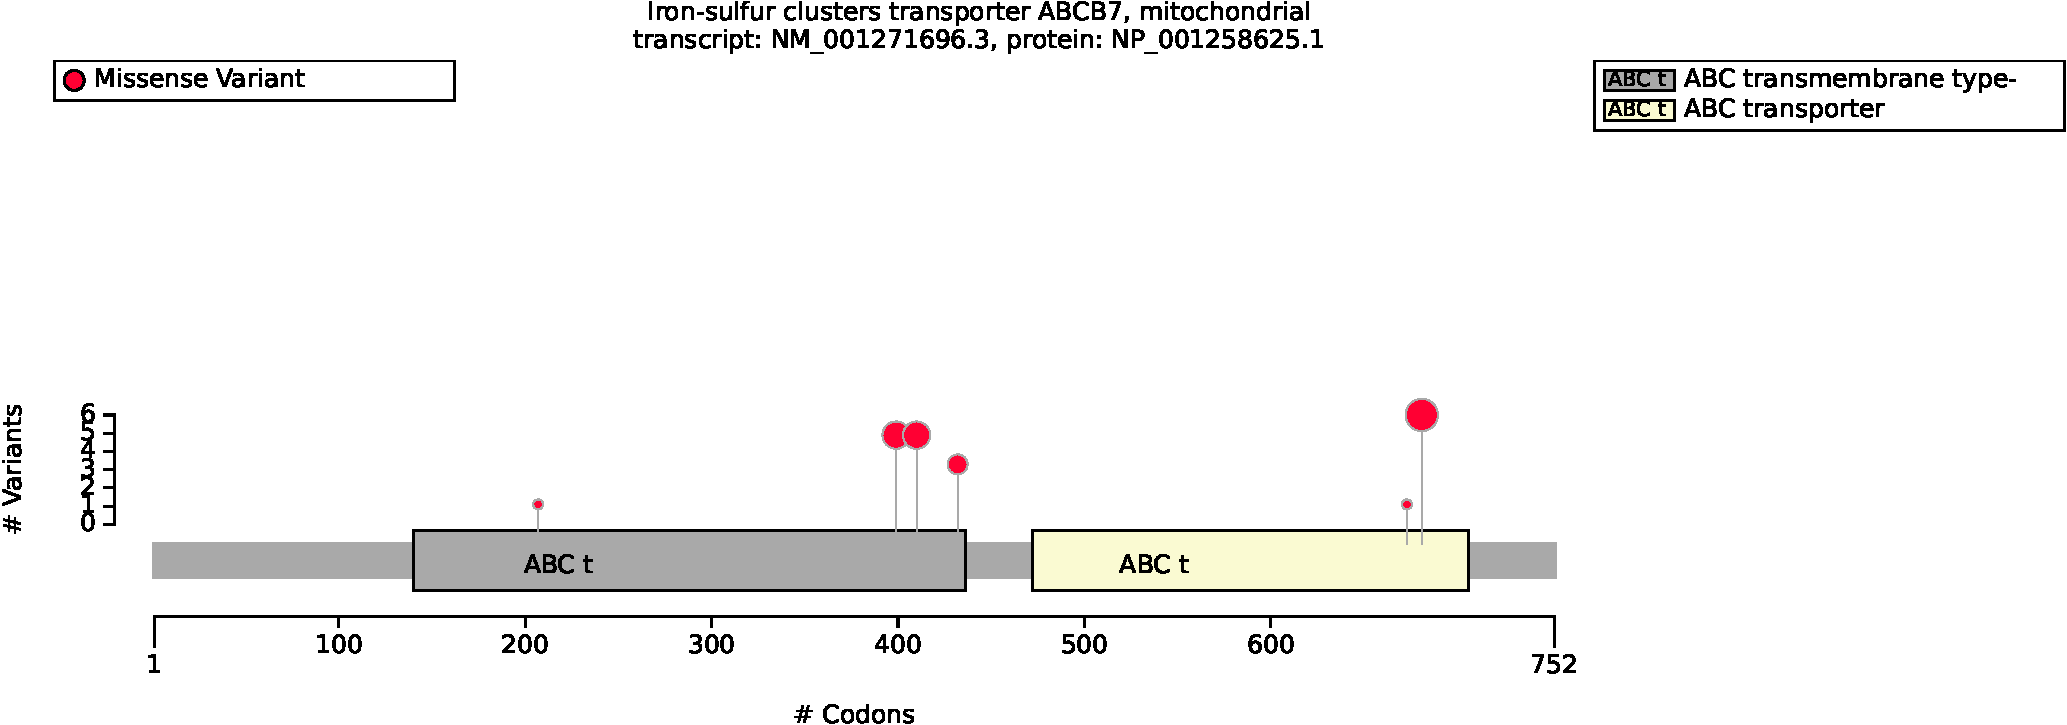
\includegraphics[width=\textwidth]{ img/ABCB7_protein_diagram.pdf} 
\captionsetup{justification=raggedright,singlelinecheck=false}
\caption{Distribution of variants in ABCB7}
\end{subfigure}

\vspace{2em}

\begin{subfigure}[b]{0.95\textwidth}
\centering
\resizebox{\textwidth}{!}{
\begin{tabular}{llllrr}
\toprule
Genotype (A) & Genotype (B) & total tests performed & significant results\\
\midrule
ABC transmembrane type-1 & Other region & 12 & 0\\
p.Gly682Ser & Other variant & 10 & 0\\
\bottomrule
\end{tabular}
}
\captionsetup{justification=raggedright,singlelinecheck=false}
\caption{Fisher Exact Test performed to compare HPO annotation frequency with respect to variants located in the
ABC transmembrane type-1 region and p.Gly682Ser.}
\end{subfigure}

\vspace{2em}

\caption{ The cohort comprised 18 individuals (0 females, 18 males). A total of 52 HPO terms were used to annotate the cohort. Disease diagnosis: Anemia, sideroblastic, and spinocerebellar ataxia (OMIM:301310). No statistically significant results identified. A total of 18 unique variant alleles were found in \textit{ABCB7} (transcript: \texttt{NM\_001271696.3}, protein id: \texttt{NP\_001258625.1}).}
\end{figure}

\begin{figure}[htbp]
    \centering
    \begin{subfigure}[b]{0.95\textwidth}
    \centering
    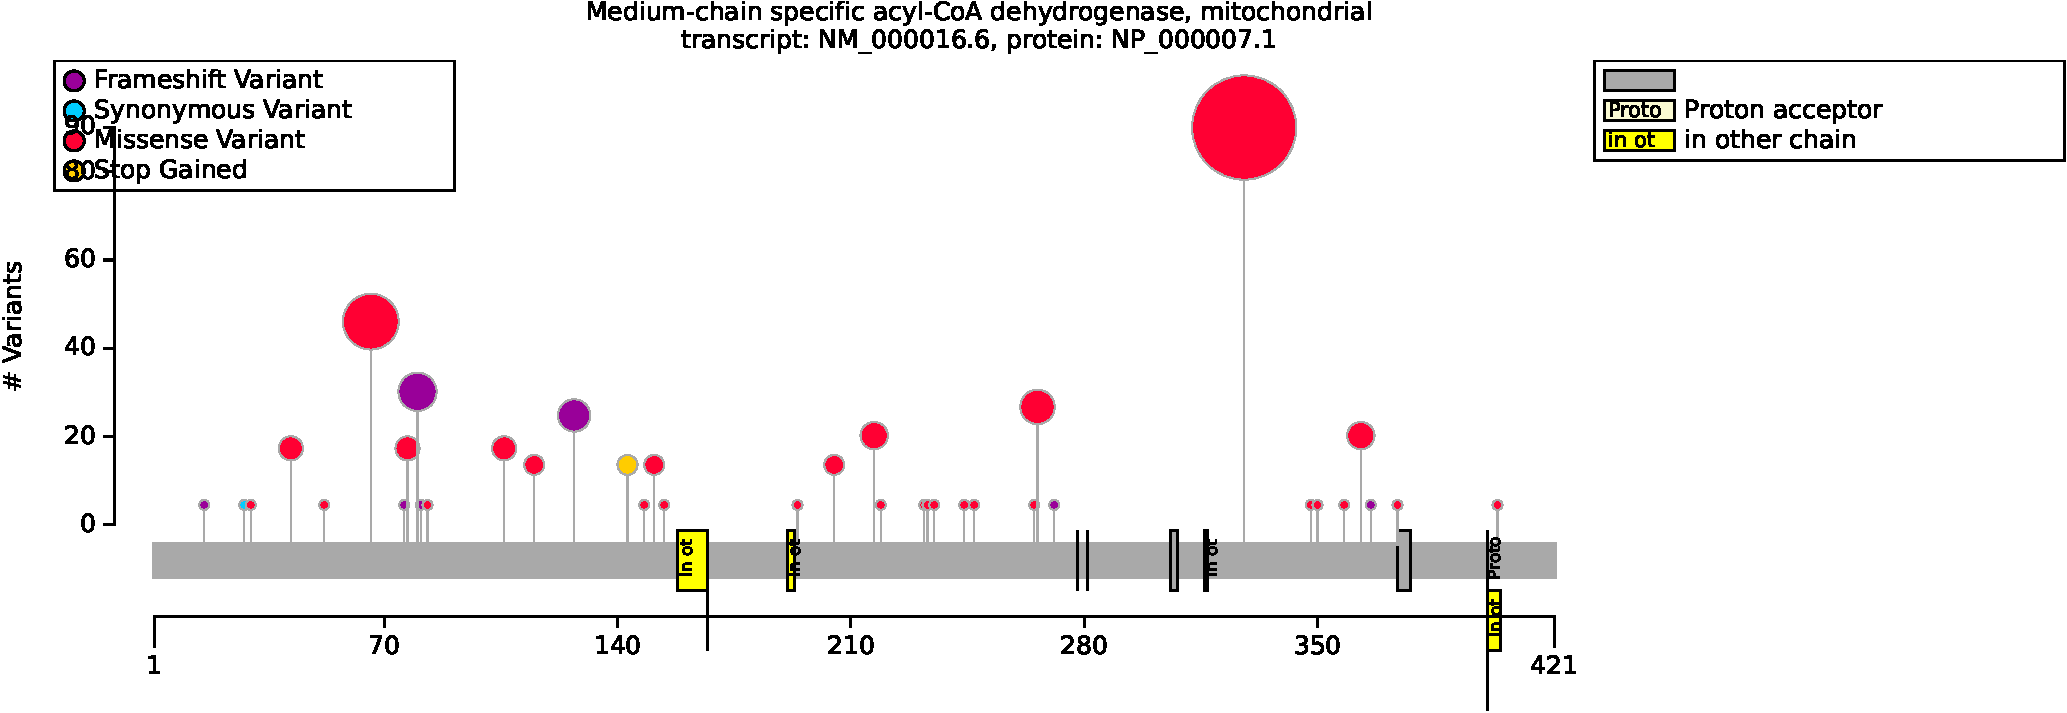
\includegraphics[width=\textwidth]{ img/ACADM_protein_diagram.pdf} 
    \captionsetup{justification=raggedright,singlelinecheck=false}
    \caption{Distribution of variants in ACADM}
    \end{subfigure}
    
    \vspace{2em}

    \begin{subfigure}[b]{0.95\textwidth}
    \centering
    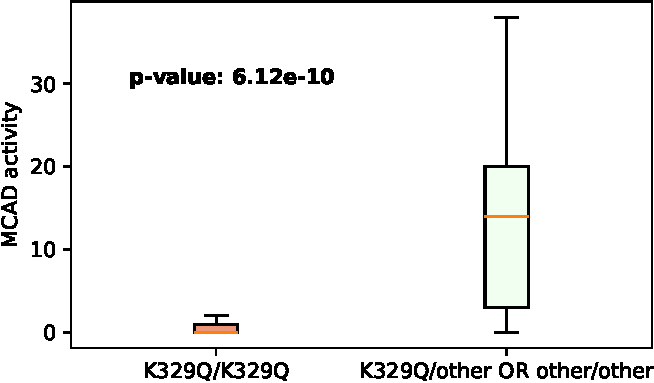
\includegraphics[width=0.3\textwidth]{ img/acadm_k329q.pdf} 
    \captionsetup{justification=raggedright,singlelinecheck=false}
    \caption{Lys329Glu: t test for MCAD Activity (\% normal; LOINC:74892-1): p=$6.12\times 10^{-10}$.}
    \end{subfigure}
    
    \vspace{2em}
    
    \begin{subfigure}[b]{0.95\textwidth}
    \captionsetup{justification=raggedright,singlelinecheck=false}
    \resizebox{\textwidth}{!}{
    \begin{tabular}{llllrr}
    \toprule
    Description & Variable & Genotype (A) & Genotype (B) & p-value & xrefs\\
    \midrule
    Value of MCAD Activity\% [LOINC:74892-1] & LOINC:74892-1 & K329Q/K329Q & K329Q/other OR other/other & $6.12\times 10^{-10}$ & \cite{PMID_33580884}\\
    \bottomrule
    \end{tabular}
    }
    \caption{t-test to compare K329Q/K329Q and K329Q/other OR other/other with respect to LOINC:74892-1. Mean MCAD activity for K329/K329: 0.52\%, and for K329/other or other/other: 13.23\% }
    \end{subfigure}
    
    \vspace{2em}
    
    \begin{subfigure}[b]{0.95\textwidth}
    \captionsetup{justification=raggedright,singlelinecheck=false}
    \resizebox{\textwidth}{!}{
    \begin{tabular}{llllrr}
    \toprule
    Description & Variable & Genotype (A) & Genotype (B) & p-value & xrefs\\
    \midrule
    Value of MCAD Activity\% [LOINC:74892-1] & LOINC:74892-1 & Y67H/Y67H OR Y67H/other & other/other & $2.01\times 10^{-5}$ & \cite{PMID_33580884}\\
    \bottomrule
    \end{tabular}
    }
    \caption{t-test to compare Y67H/Y67H OR Y67H/other and other/other with respect to LOINC:74892-1. Mean MCAD activity for Y67H/Y67H: 18.60\%, and for Y67H/other or other/other: 7.68\% }
    \end{subfigure}
    
    \vspace{2em}
    
    \caption{The cohort comprised 115 individuals (0 females, 0 males, 115 with unknown sex). The cohort had data about  medium chain Acyl-CoA dehydrogenase (MCAD), expressed as percentage of normal.
    The variant c.985G$>$A (p.Lys329Glu) is known to be severe, and the variant c.199T$>$C (p.Tyr67His) is known to be mild \cite{PMID_33580884}.
    Disease diagnosis: Acyl-CoA dehydrogenase, medium chain, deficiency of (OMIM:201450). No statistically significant results identified. A total of 188 unique variant alleles were found in \textit{ACADM} (transcript: \texttt{NM\_000016.6}, protein id: \texttt{NP\_000007.1}).}
    \end{figure}
    
\begin{figure}[htbp]
\centering
\begin{subfigure}[b]{0.95\textwidth}
\centering
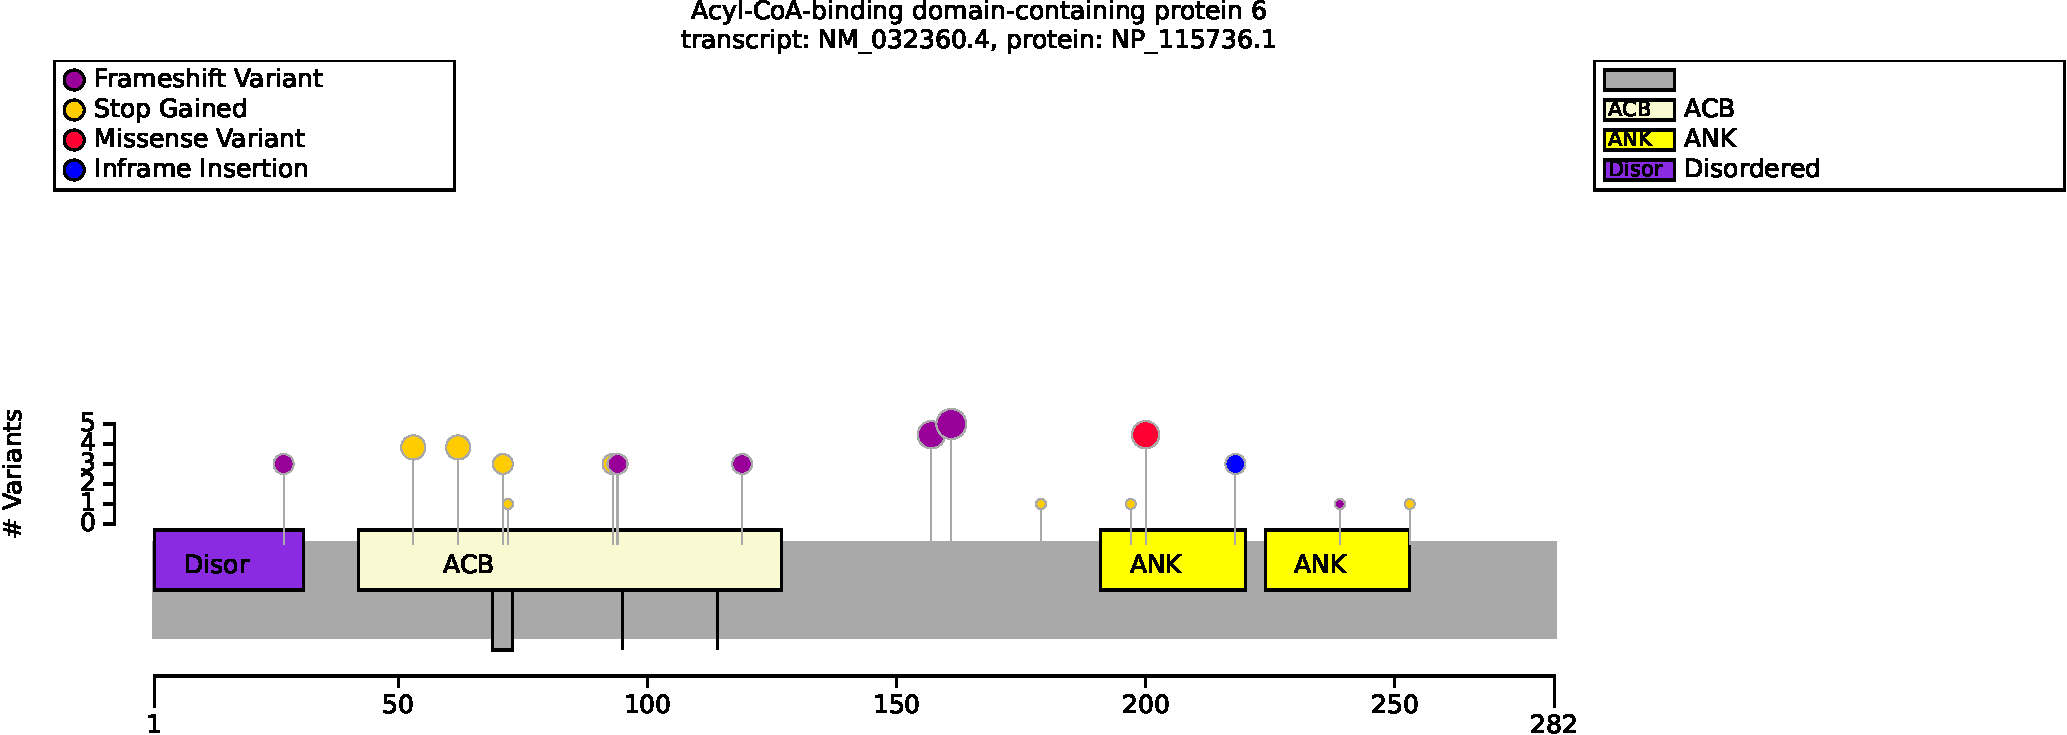
\includegraphics[width=\textwidth]{ img/ACBD6_protein_diagram.pdf} 
\captionsetup{justification=raggedright,singlelinecheck=false}
\caption{Distribution of variants in ACBD6}
\end{subfigure}

\vspace{2em}

\begin{subfigure}[b]{0.95\textwidth}
\centering
\resizebox{\textwidth}{!}{
\begin{tabular}{llllrr}
\toprule
Genotype (A) & Genotype (B) & total tests performed & significant results\\
\midrule
missense/missense OR missense/other & other/other & 52 & 0\\
\bottomrule
\end{tabular}
}
\captionsetup{justification=raggedright,singlelinecheck=false}
\caption{         Fisher Exact Test performed to compare HPO annotation frequency with respect to missense/missense OR missense/other and other/other. }
\end{subfigure}

\vspace{2em}

\begin{subfigure}[b]{0.95\textwidth}
\centering
\resizebox{\textwidth}{!}{
\begin{tabular}{llllrr}
\toprule
Genotype (A) & Genotype (B) & total tests performed & significant results\\
\midrule
ACB/ACB OR ACB/other & other/other & 50 & 0\\
\bottomrule
\end{tabular}
}
\captionsetup{justification=raggedright,singlelinecheck=false}
\caption{Fisher Exact Test performed to compare HPO annotation frequency with respect to ACB/ACB OR ACB/other and other/other. }
\end{subfigure}

\vspace{2em}

\begin{subfigure}[b]{0.95\textwidth}
\centering
\resizebox{\textwidth}{!}{
\begin{tabular}{llllrr}
\toprule
Genotype (A) & Genotype (B) & total tests performed & significant results\\
\midrule
FEMALE & MALE & 49 & 0\\
\bottomrule
\end{tabular}
}
\captionsetup{justification=raggedright,singlelinecheck=false}
\caption{Fisher Exact Test performed to compare HPO annotation frequency with respect to FEMALE and MALE.}
\end{subfigure}

\vspace{2em}

\caption{The cohort comprised 45 individuals (22 females, 23 males). A total of 79 HPO terms were used to annotate the cohort. Disease diagnosis: Neurodevelopmental disorder with progressive movement abnormalities (OMIM:620785). No statistically significant results identified. A total of 45 unique variant alleles were found in \textit{ACBD6} (transcript: \texttt{NM\_032360.4}, protein id: \texttt{NP\_115736.1}).}
\end{figure}

\begin{figure}[htbp]
\centering
\begin{subfigure}[b]{0.95\textwidth}
\centering
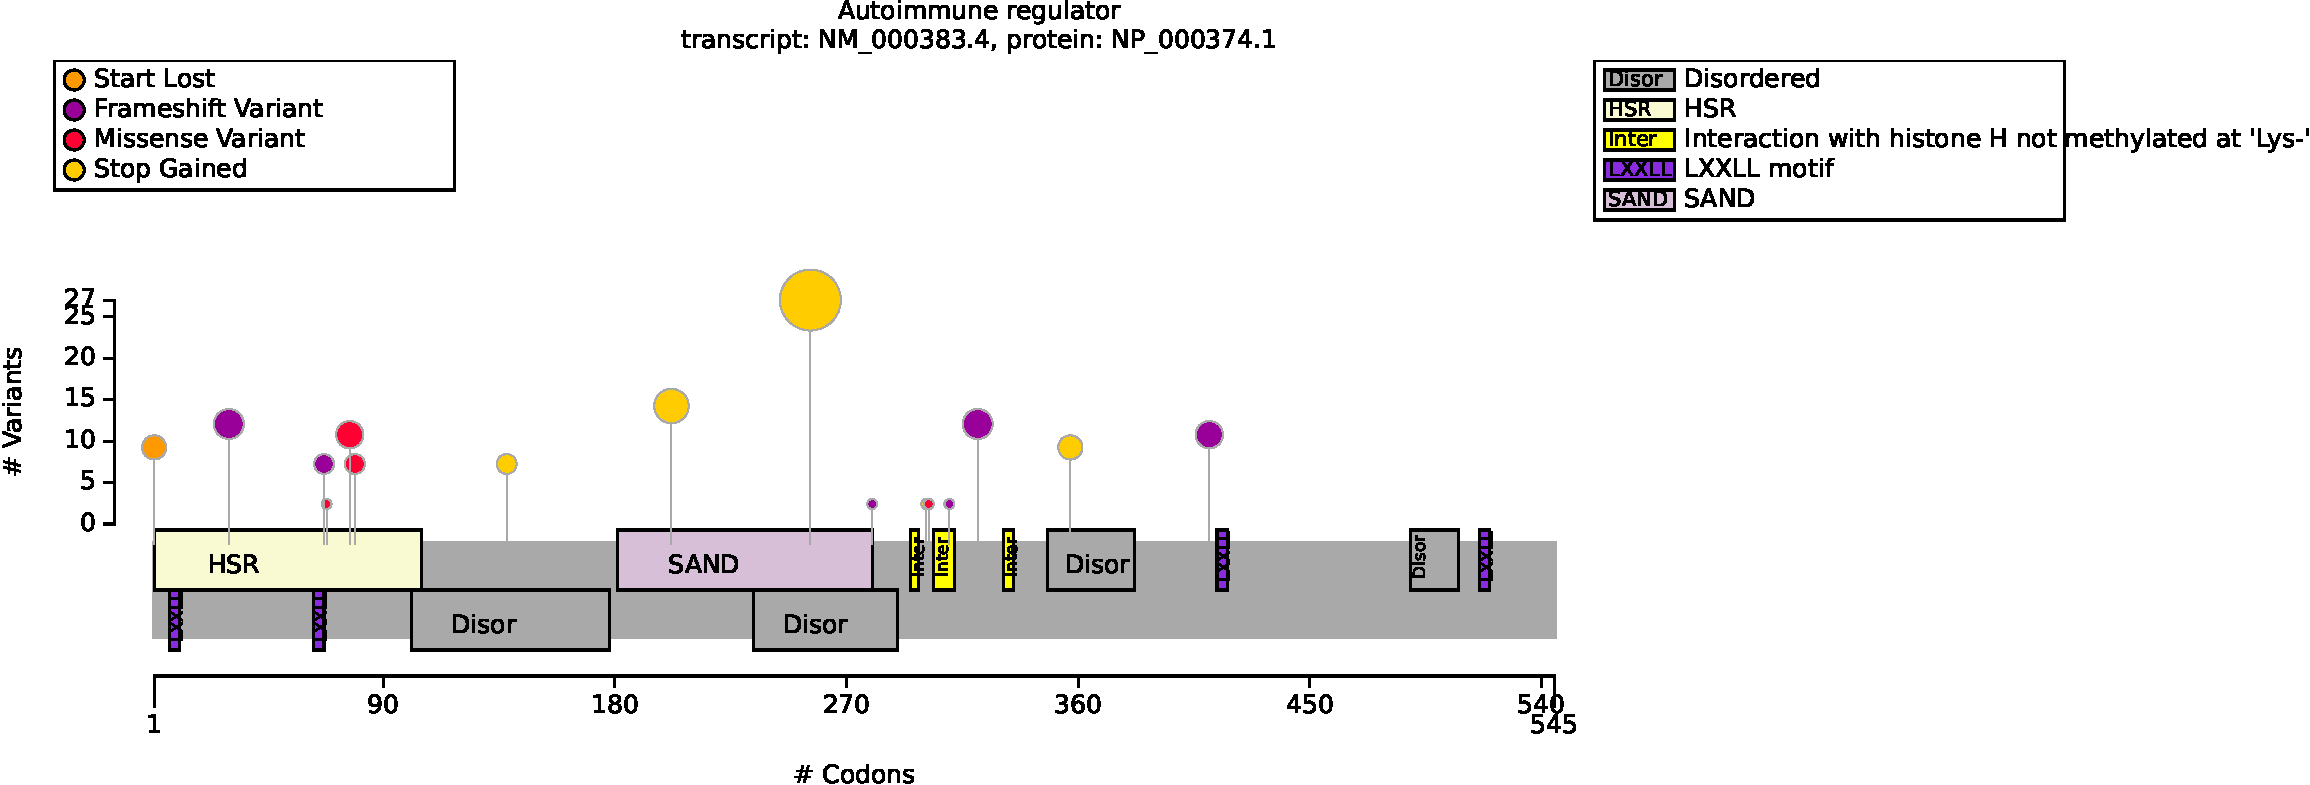
\includegraphics[width=\textwidth]{ img/AIRE_protein_diagram.pdf} 
\captionsetup{justification=raggedright,singlelinecheck=false}
\caption{Distribution of variants in AIRE}
\end{subfigure}

\vspace{2em}

\begin{subfigure}[b]{0.95\textwidth}
\centering
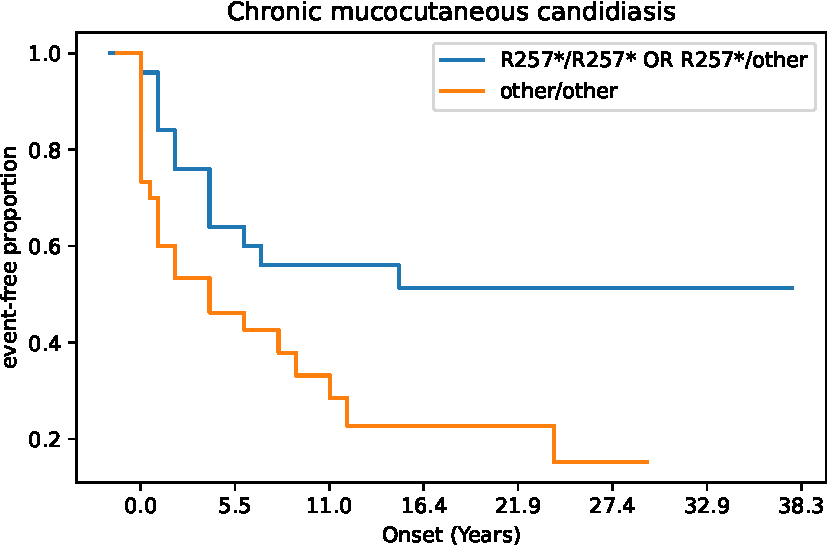
\includegraphics[width=0.3\textwidth]{ img/AIRE_cmc.pdf} 
\captionsetup{justification=raggedright,singlelinecheck=false}
\caption{print("log-rank p-value for Chronic mucocutaneous candidiasis (HP:0002728) and R357*/R357* or R357*/other versus other/other 0.0192")}
\end{subfigure}
    
\vspace{2em}

\begin{subfigure}[b]{0.95\textwidth}
\centering
\resizebox{\textwidth}{!}{
\begin{tabular}{llllrr}
\toprule
Genotype (A) & Genotype (B) & total tests performed & significant results\\
\midrule
R257*/R257* OR R257*/other & other/other & 12 & 0\\
\bottomrule
\end{tabular}
}
\captionsetup{justification=raggedright,singlelinecheck=false}
\caption{Fisher Exact Test performed to compare HPO annotation frequency with respect to R257*/R257* OR R257*/other and other/other. }
\end{subfigure}

\vspace{2em}

\begin{subfigure}[b]{0.95\textwidth}
\captionsetup{justification=raggedright,singlelinecheck=false}
\resizebox{\textwidth}{!}{
\begin{tabular}{llllrr}
\toprule
Description & Variable & Genotype (A) & Genotype (B) & p-value & xrefs\\
\midrule
Survival analysis: Chronic mucocutaneous candidiasis & Onset of HP:0002728 & R257*/R257* OR R257*/other & other/other & 0.019 & -\\
\bottomrule
\end{tabular}
}
\caption{ Onset of Chronic mucocutaneous candidiasis to compare R257*/R257* OR R257*/other and other/other with respect to Onset of HP:0002728. }
\end{subfigure}

\vspace{2em}

\caption{ The cohort comprised 58 individuals (31 females, 27 males). 2 of these individuals were reported to be deceased. A total of 47 HPO terms were used to annotate the cohort. Disease diagnosis: Autoimmune polyendocrinopathy syndrome , type I, with or without reversible metaphyseal dysplasia (OMIM:240300). A
 higher prevalence of chronic mucocutanous candidiasis with the variant Arg357Ter than with other variants was reported previously \cite{PMID_12050215}. We did not identify a significant difference in prevalence A total of 70 unique variant alleles were found in \textit{AIRE} (transcript: \texttt{NM\_000383.4}, protein id: \texttt{NP\_000374.1}).}
\end{figure}

\begin{figure}[htbp]
\section*{ANKRD11}
\centering
\begin{subfigure}[b]{0.95\textwidth}
\centering
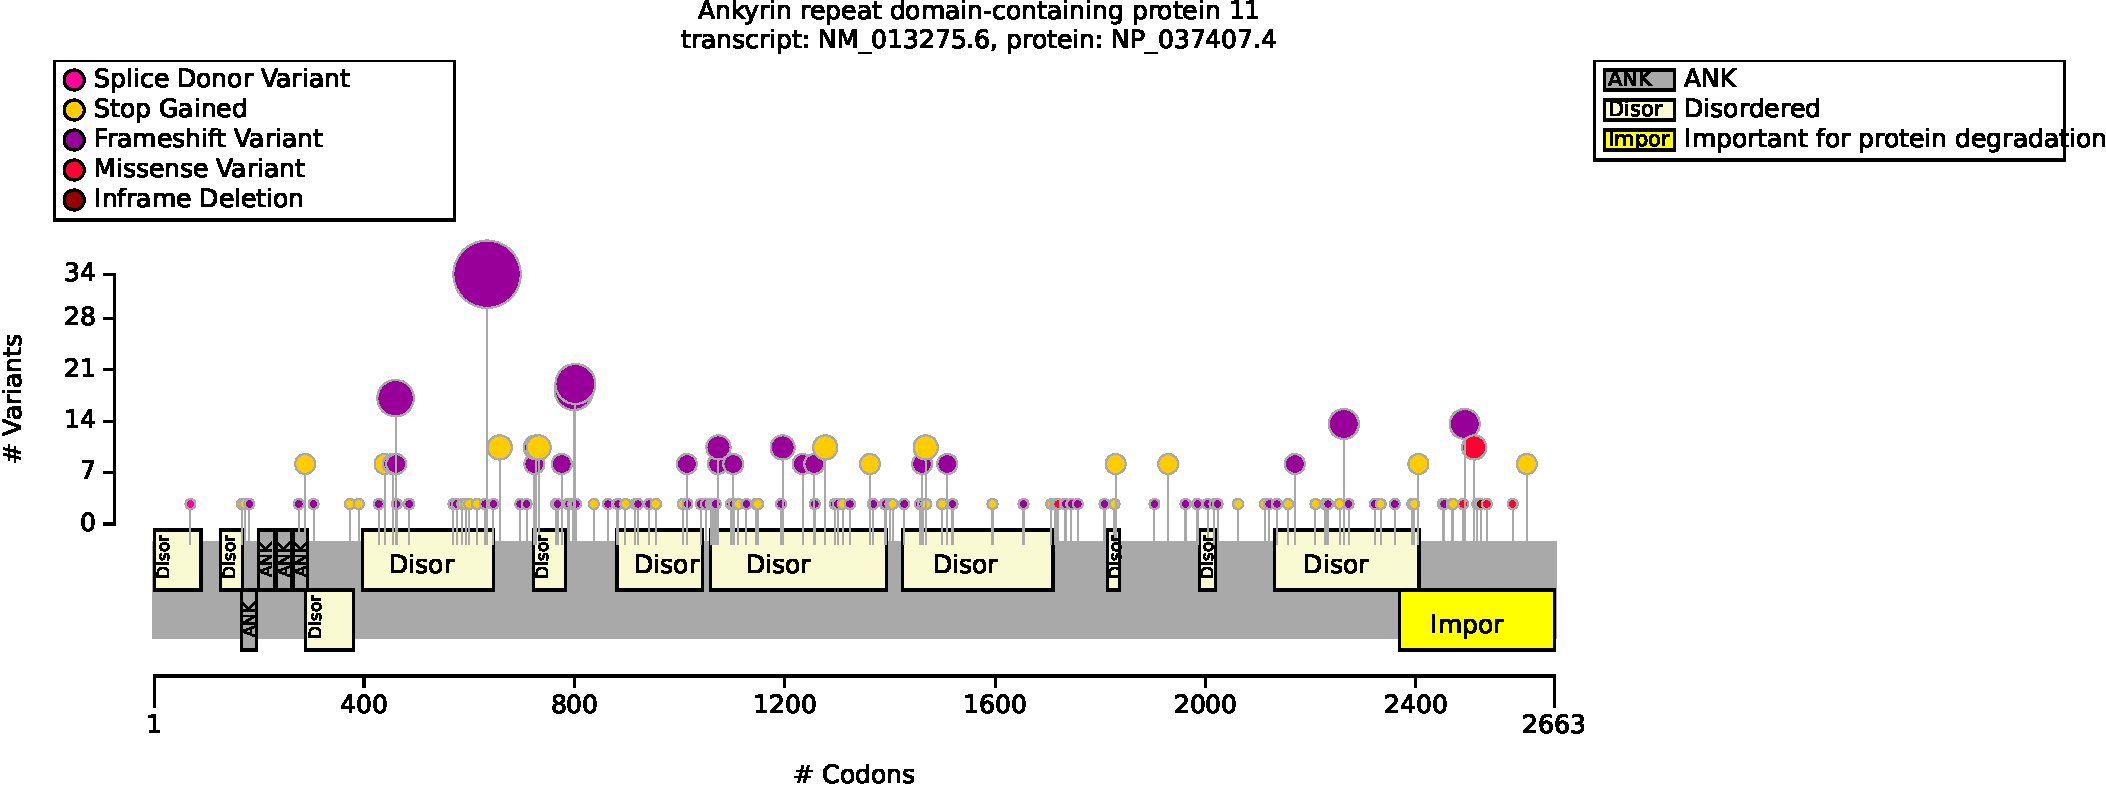
\includegraphics[width=\textwidth]{ img/ANKRD11_protein_diagram.pdf} 
\captionsetup{justification=raggedright,singlelinecheck=false}
\caption{Distribution of variants in ANKRD11}
\end{subfigure}

\vspace{2em}

\begin{subfigure}[b]{0.95\textwidth}
\centering
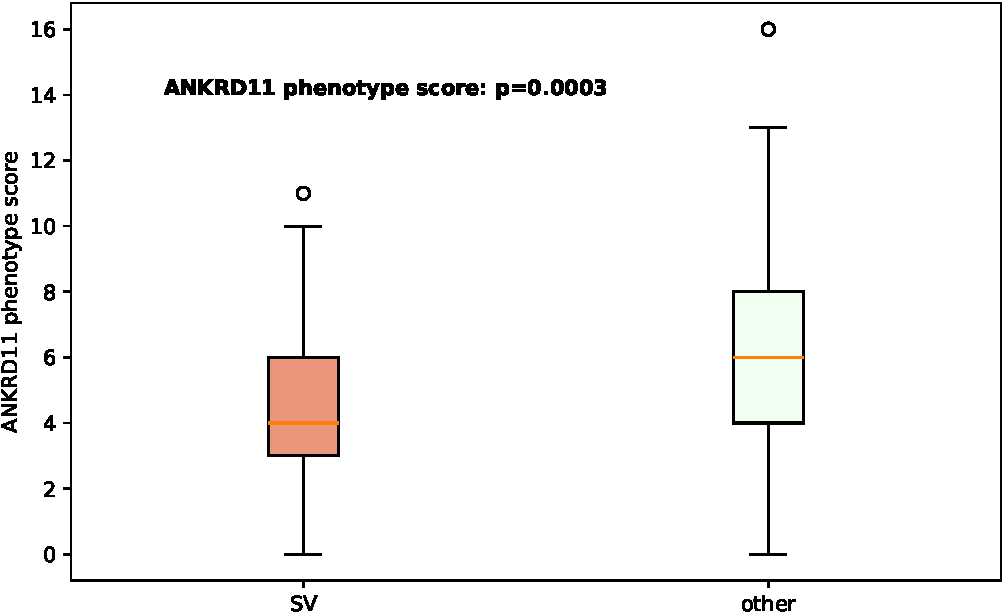
\includegraphics[width=0.3\textwidth]{ img/ANKRD11_phenoscore.pdf} 
\captionsetup{justification=raggedright,singlelinecheck=false}
\caption{ANKRD11 phenotypical score. Mean for structural variants: 4.62, and for other variants: 5.94}
\end{subfigure}

\vspace{2em}

\begin{subfigure}[b]{0.95\textwidth}
\centering
\resizebox{\textwidth}{!}{
\begin{tabular}{llllrr}
\toprule
Genotype (A) & Genotype (B) & total tests performed & significant results\\
\midrule
SV & other & 23 & 0\\
exon 9 & other & 23 & 0\\
c.1903\_1907del & other & 23 & 0\\
\bottomrule
\end{tabular}
}
\captionsetup{justification=raggedright,singlelinecheck=false}
\caption{Fisher Exact Test performed to compare HPO annotation frequency with respect to SV, exon 9, and c.1903\_1907del.}
\end{subfigure}

\vspace{2em}

\begin{subfigure}[b]{0.95\textwidth}
\captionsetup{justification=raggedright,singlelinecheck=false}
\resizebox{\textwidth}{!}{
\begin{tabular}{llllrr}
\toprule
Description & Variable & Genotype (A) & Genotype (B) & p-value & xrefs\\
\midrule
ANKRD11 phenotype score & HPO group count & SV & other & $2.64\times 10^{-4}$ & \cite{PMID_36446582}\\
ANKRD11 phenotype score & HPO group count & FEMALE & MALE & 0.0075 & -\\

\bottomrule
\end{tabular}
}
\caption{AKKRD11 phenotype score for structural variants: 4.62; other variants: 5.94. male/female comparison: Female 5.28, Male: 6.15.}
\end{subfigure}

\vspace{2em}

\caption{The cohort comprised 337 individuals (143 females, 175 males, 19 with unknown sex). A total of 48 HPO terms were used to annotate the cohort. Disease diagnosis: KBG syndrome (OMIM:148050). Validated results on ANKRD11 phenotypical score. Other results did not survive multiple testing correction. Awamleh et al. (2023) stated that no significant DNAm differences based on sex at the identified KBGS-specific signature sites \cite{PMID_36440975}. We are aware of no other publication that mentions sex-specific differences in KBGS. A total of 163 unique variant alleles were found in \textit{ANKRD11} (transcript: \texttt{NM\_013275.6}, protein id: \texttt{NP\_037407.4}).}
\end{figure}

\begin{figure}[htbp]
\centering
\begin{subfigure}[b]{0.95\textwidth}
\centering
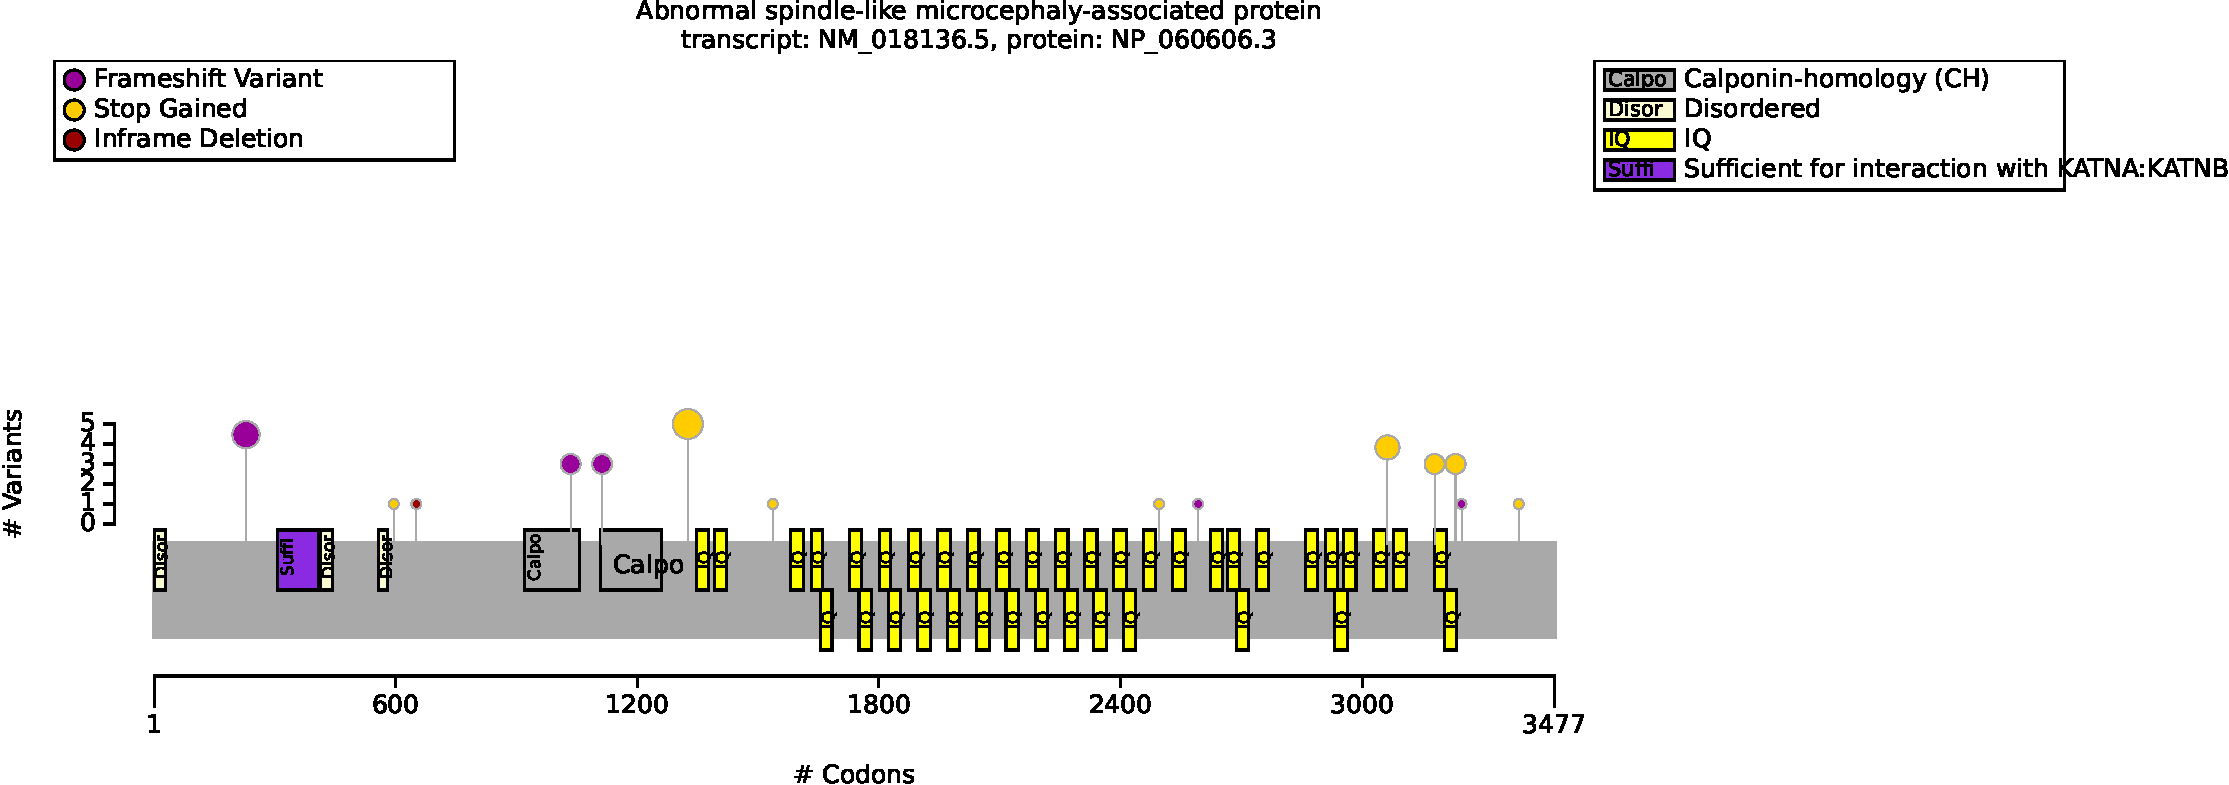
\includegraphics[width=\textwidth]{ img/ASPM_protein_diagram.pdf} 
\captionsetup{justification=raggedright,singlelinecheck=false}
\caption{Distribution of variants in ASPM}
\end{subfigure}

\vspace{2em}

\begin{subfigure}[b]{0.95\textwidth}
\centering
\resizebox{\textwidth}{!}{
\begin{tabular}{llllrr}
\toprule
Genotype (A) & Genotype (B) & total tests performed & significant results\\
\midrule
N Term/N Term OR N Term/other & other/other & 11 & 0\\
FEMALE & MALE & 11 & 0\\
\bottomrule
\end{tabular}
}
\captionsetup{justification=raggedright,singlelinecheck=false}
\caption{Fisher Exact Test performed to compare HPO annotation frequency with respect to N Term/N Term OR N Term/other and other/other, as well as male/female comparison. }
\end{subfigure}

\vspace{2em}

\caption{ The cohort comprised 22 individuals (14 females, 8 males). A total of 17 HPO terms were used to annotate the cohort. Disease diagnosis: Microcephaly 5, primary, autosomal recessive (OMIM:608716). No statistically significant results identified. A total of 28 unique variant alleles were found in \textit{ASPM} (transcript: \texttt{NM\_018136.5}, protein id: \texttt{NP\_060606.3}).}
\end{figure}

%% todo
\begin{figure}[htbp]
\centering
\begin{subfigure}[b]{0.95\textwidth}
\centering
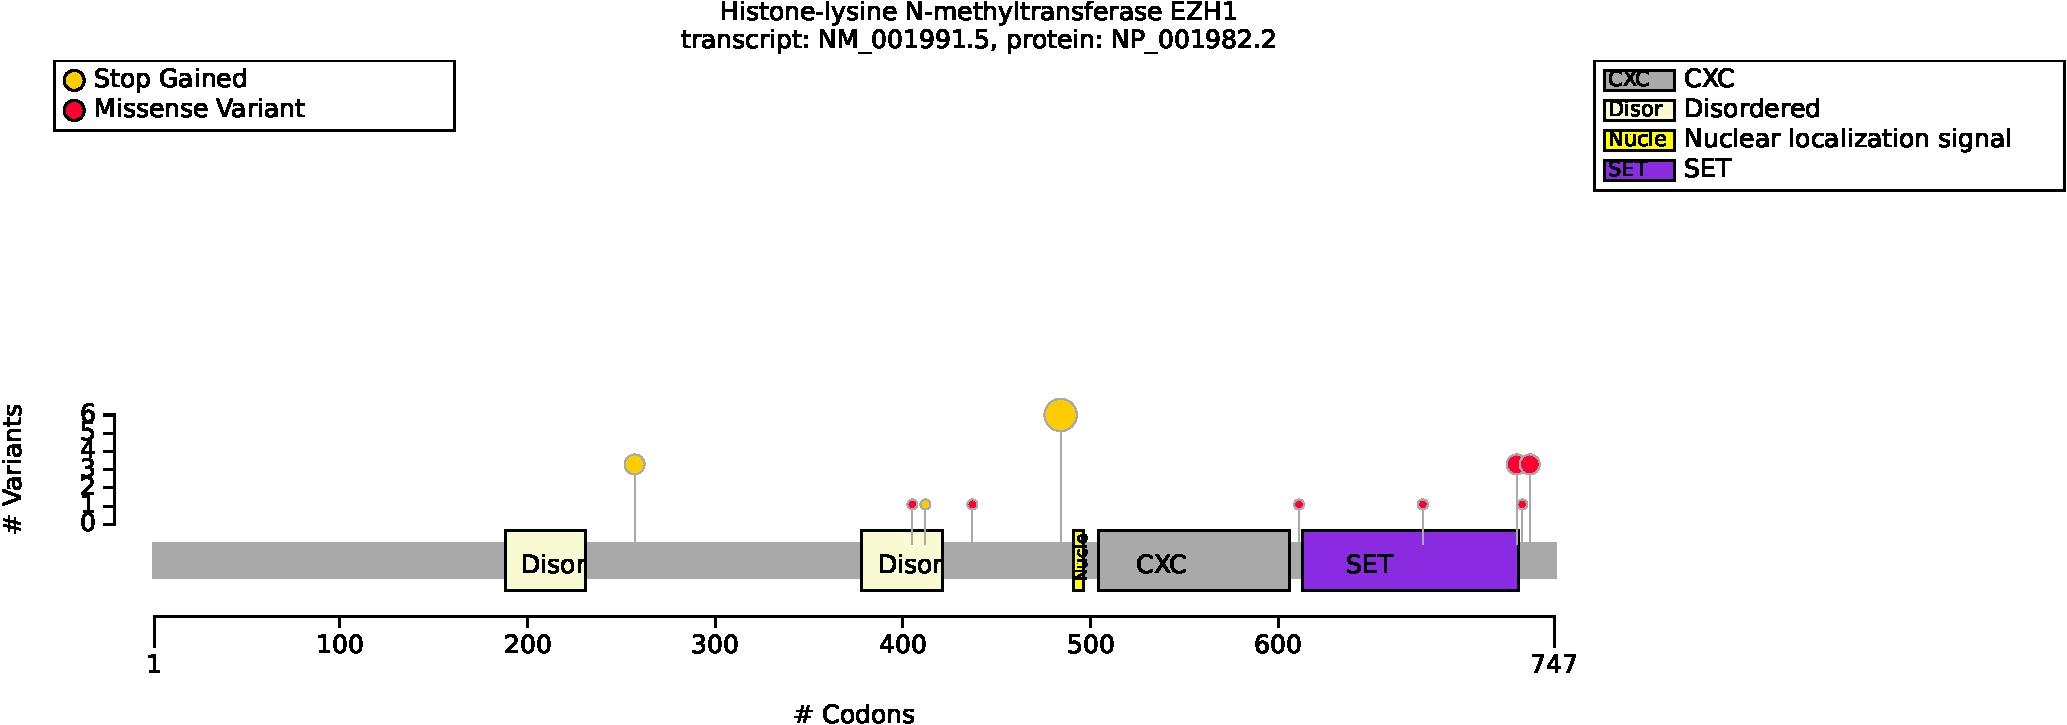
\includegraphics[width=\textwidth]{ img/EZH1_protein_diagram.pdf} 
\captionsetup{justification=raggedright,singlelinecheck=false}
\caption{Distribution of variants in EZH1}
\end{subfigure}

\vspace{2em}

\begin{subfigure}[b]{0.95\textwidth}
\centering
\resizebox{\textwidth}{!}{
\begin{tabular}{llllrr}
\toprule
Genotype (A) & Genotype (B) & total tests performed & significant results\\
\midrule
1 allele & 2 alleles & 23 & 0\\
\bottomrule
\end{tabular}
}
\captionsetup{justification=raggedright,singlelinecheck=false}
\caption{Fisher Exact Test performed to compare HPO annotation frequency with respect to monoallelic and biallelic pathogenic variants. }
\end{subfigure}

\vspace{2em}

\caption{The cohort comprised 19 individuals (10 females, 8 males, 1 with unknown sex). A total of 106 HPO terms were used to annotate the cohort. Disease diagnosis: EZH1-related neurodevelopmental disorder (OMIM:601674). No statistically significant results identified. A total of 20 unique variant alleles were found in \textit{EZH1} (transcript: \texttt{NM\_001991.5}, protein id: \texttt{NP\_001982.2}). In the original publication, it is stated that patients show neurodevelopmental delay with variable clinical presentations regardless of variant type and zygosity \cite{PMID_37433783}.}
\end{figure}

%% todo

\begin{figure}[htbp]
\centering
\begin{subfigure}[b]{0.95\textwidth}
\centering
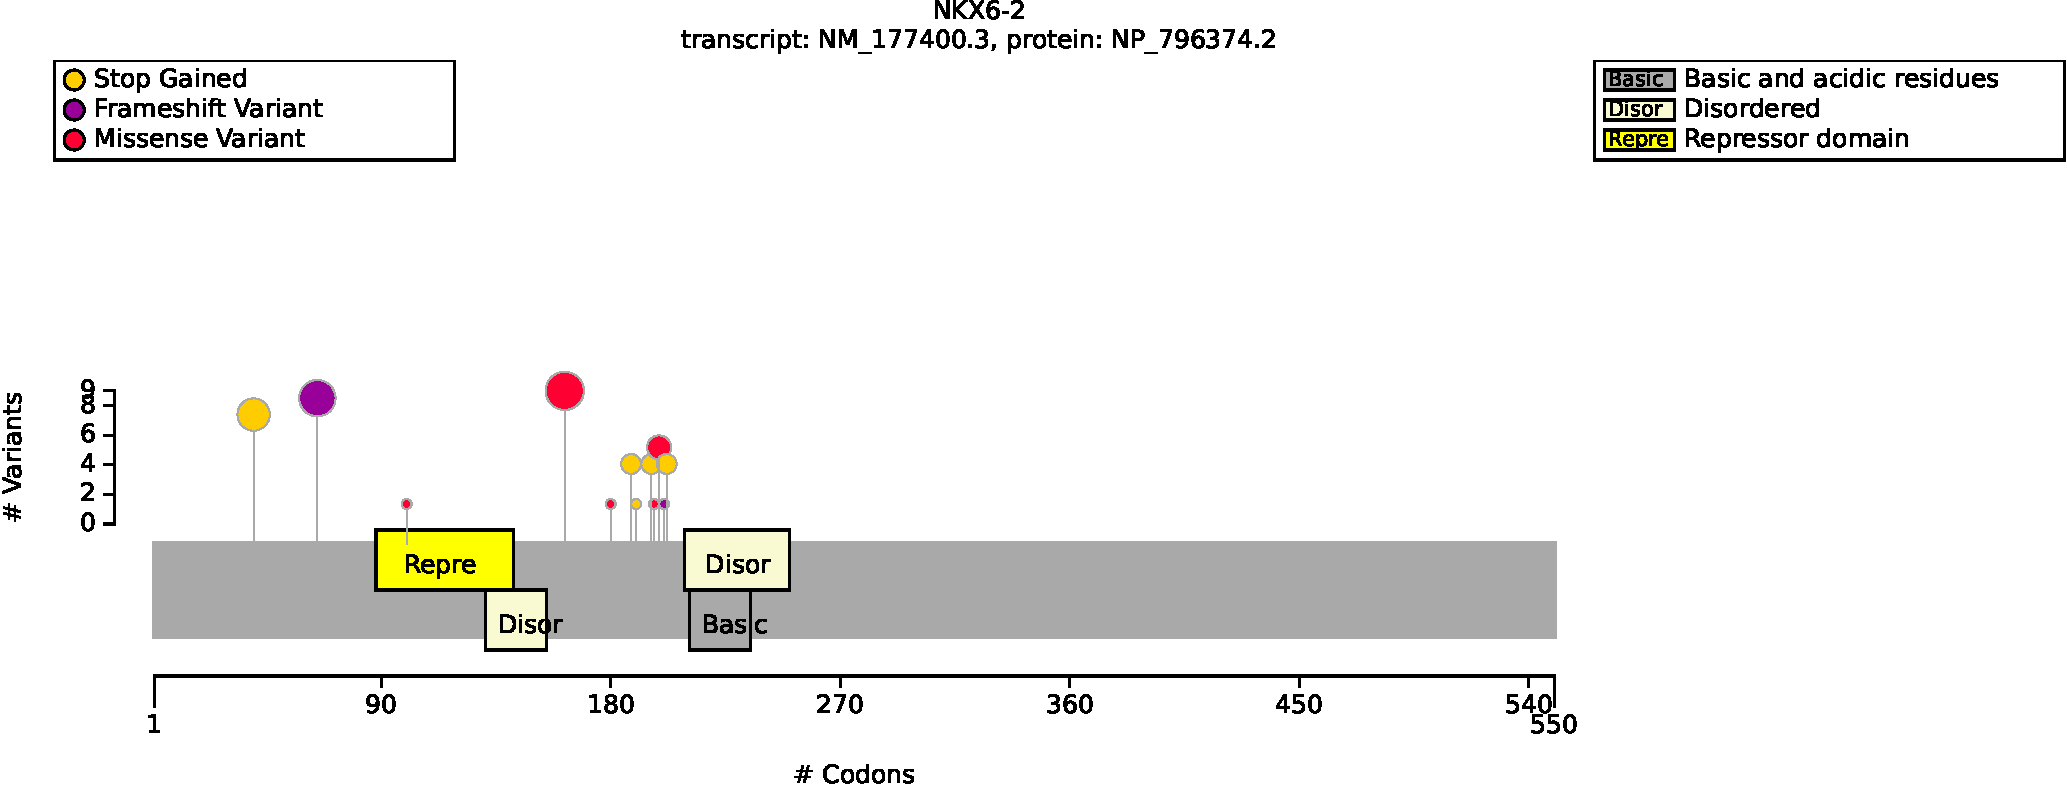
\includegraphics[width=\textwidth]{ img/NKX6-2_protein_diagram.pdf} 
\captionsetup{justification=raggedright,singlelinecheck=false}
\caption{Distribution of variants in NKX6-2}
\end{subfigure}

\vspace{2em}

\begin{subfigure}[b]{0.95\textwidth}
\centering
\resizebox{\textwidth}{!}{
\begin{tabular}{llllrr}
\toprule
Genotype (A) & Genotype (B) & total tests performed & significant results\\
\midrule
missense/missense & other/other OR missense/other & 18 & 0\\
L163V/L163V & L163V/other OR other/other & 18 & 0\\
N term/N term OR N term/other & other/other & 20 & 0\\
FEMALE & MALE & 20 & 0\\
\bottomrule
\end{tabular}
}
\captionsetup{justification=raggedright,singlelinecheck=false}
\caption{Fisher Exact Test performed to compare HPO annotation frequency. }
\end{subfigure}

\vspace{2em}

\caption{The cohort comprised 33 individuals (15 females, 18 males). A total of 39 HPO terms were used to annotate the cohort. Disease diagnosis: Spastic ataxia 8, autosomal recessive, with hypomyelinating leukodystrophy (OMIM:617560). No statistically significant results identified. A total of 37 unique variant alleles were found in \textit{NKX6-2} (transcript: \texttt{NM\_177400.3}, protein id: \texttt{NP\_796374.2}).}
\end{figure}

\begin{figure}[htbp]
\centering
\begin{subfigure}[b]{0.95\textwidth}
\centering
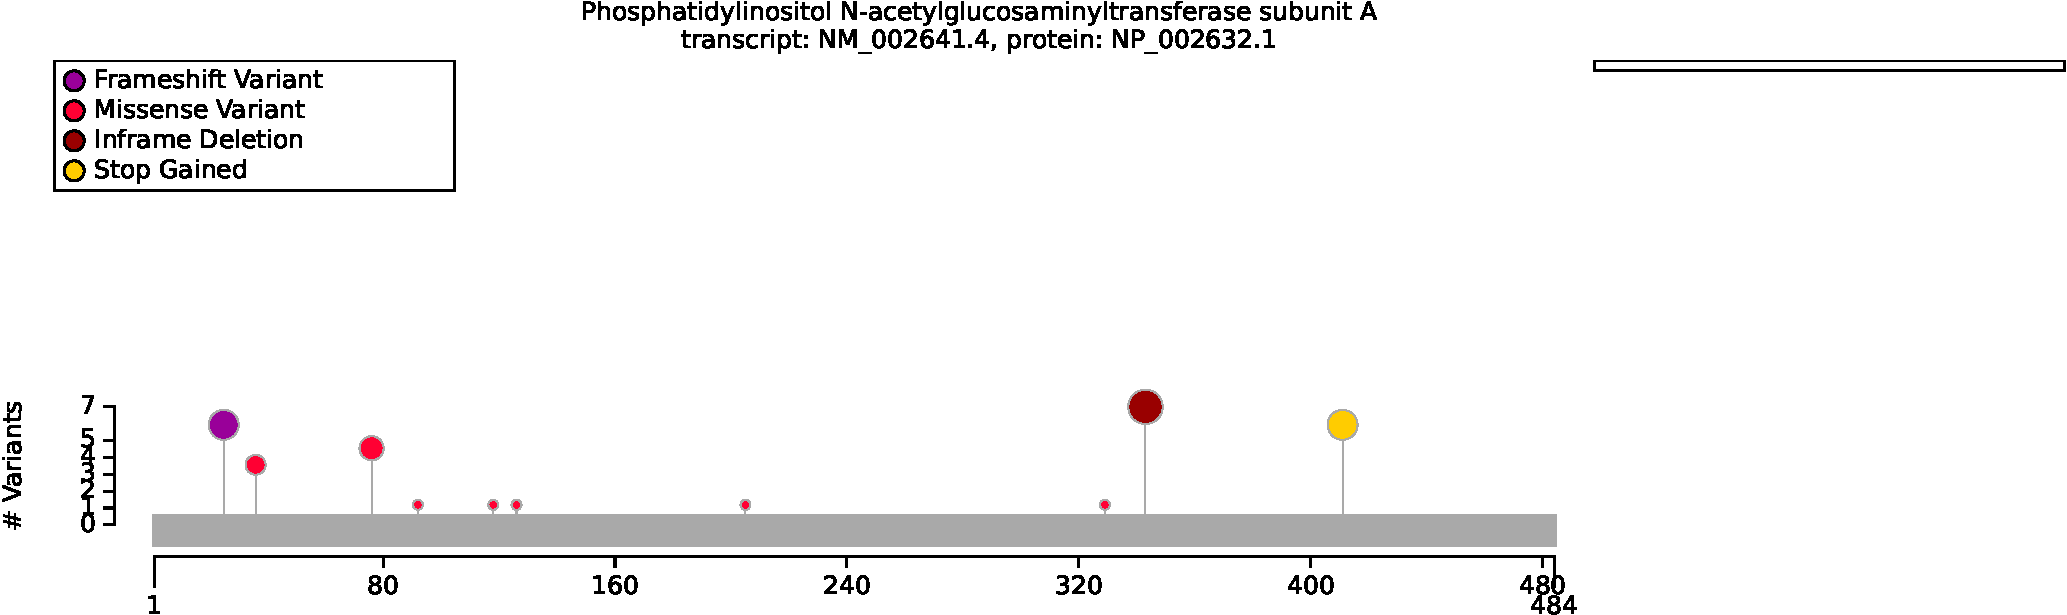
\includegraphics[width=\textwidth]{ img/PIGA_protein_diagram.pdf} 
\captionsetup{justification=raggedright,singlelinecheck=false}
\caption{Distribution of variants in PIGA}
\end{subfigure}

\vspace{2em}

\begin{subfigure}[b]{0.95\textwidth}
\centering
\resizebox{\textwidth}{!}{
\begin{tabular}{llllrr}
\toprule
Genotype (A) & Genotype (B) & total tests performed & significant results\\
\midrule
missense & other & 23 & 0\\
p.Leu344del & other & 20 & 0\\
1-100 & 100+ & 23 & 0\\
\bottomrule
\end{tabular}
}
\captionsetup{justification=raggedright,singlelinecheck=false}
\caption{Fisher Exact Test performed to compare HPO annotation frequency with respect to missense, p.Leu344del, and N-terminal (1-100) and other. }
\end{subfigure}


\vspace{2em}

\caption{The cohort comprised 27 individuals (0 females, 27 males). A total of 188 HPO terms were used to annotate the cohort. Disease diagnoses: Multiple congenital anomalies-hypotonia-seizures syndrome 2 (OMIM:300868) (21 individuals), Neurodevelopmental disorder with epilepsy and hemochromatosis (OMIM:301072) (6 individuals). No statistically significant results identified. A total of 27 unique variant alleles were found in \textit{PIGA} (transcript: \texttt{NM\_002641.4}, protein id: \texttt{NP\_002632.1}).}
\end{figure}

\begin{figure}[htbp]
\section*{PPP2R1A}
\centering
\begin{subfigure}[b]{0.95\textwidth}
\centering
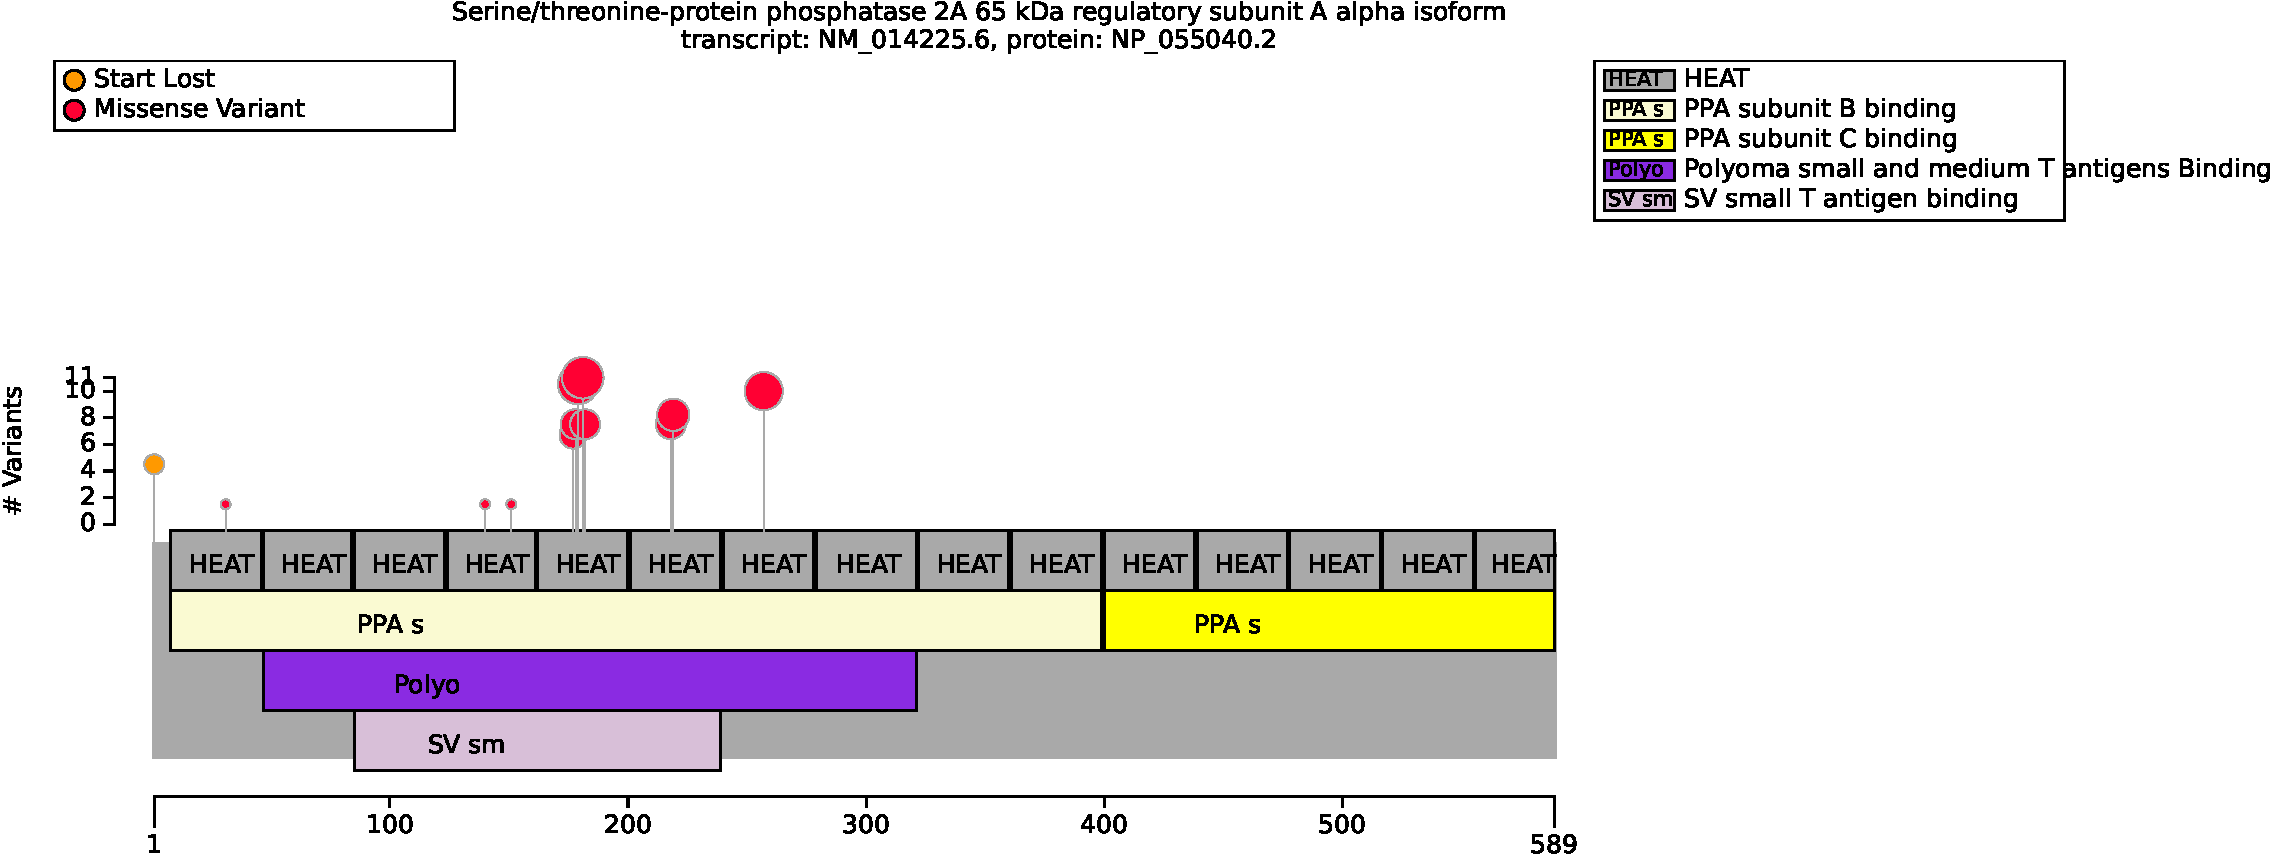
\includegraphics[width=\textwidth]{ img/PPP2R1A_protein_diagram.pdf} 
\captionsetup{justification=raggedright,singlelinecheck=false}
\caption{Distribution of variants in PPP2R1A}
\end{subfigure}

\vspace{2em}

\begin{subfigure}[b]{0.95\textwidth}
\centering
\resizebox{\textwidth}{!}{
\begin{tabular}{llllrr}
\toprule
Genotype (A) & Genotype (B) & total tests performed & significant results\\
\midrule
Absent in COSMIC & Present in COSMIC & 20 & 0\\
Arg182Trp & other & 20 & 0\\
SV40 small T antigen binding & other & 20 & 0\\
\bottomrule
\end{tabular}
}
\captionsetup{justification=raggedright,singlelinecheck=false}
\caption{             Fisher Exact Test performed to compare HPO annotation frequency with respect to genotypes. }
\end{subfigure}

\vspace{2em}

\caption{ The cohort comprised 60 individuals (24 females, 32 males, 4 with unknown sex). A total of 52 HPO terms were used to annotate the cohort. Disease diagnosis: Houge-Janssen syndrome 2 (OMIM:616362). No statistically significant results identified. A total of 60 unique variant alleles were found in \textit{PPP2R1A} (transcript: \texttt{NM\_014225.6}, protein id: \texttt{NP\_055040.2}).}
\end{figure}

\begin{figure}[htbp]
\section*{PTPN11}
\centering
\begin{subfigure}[b]{0.95\textwidth}
\centering
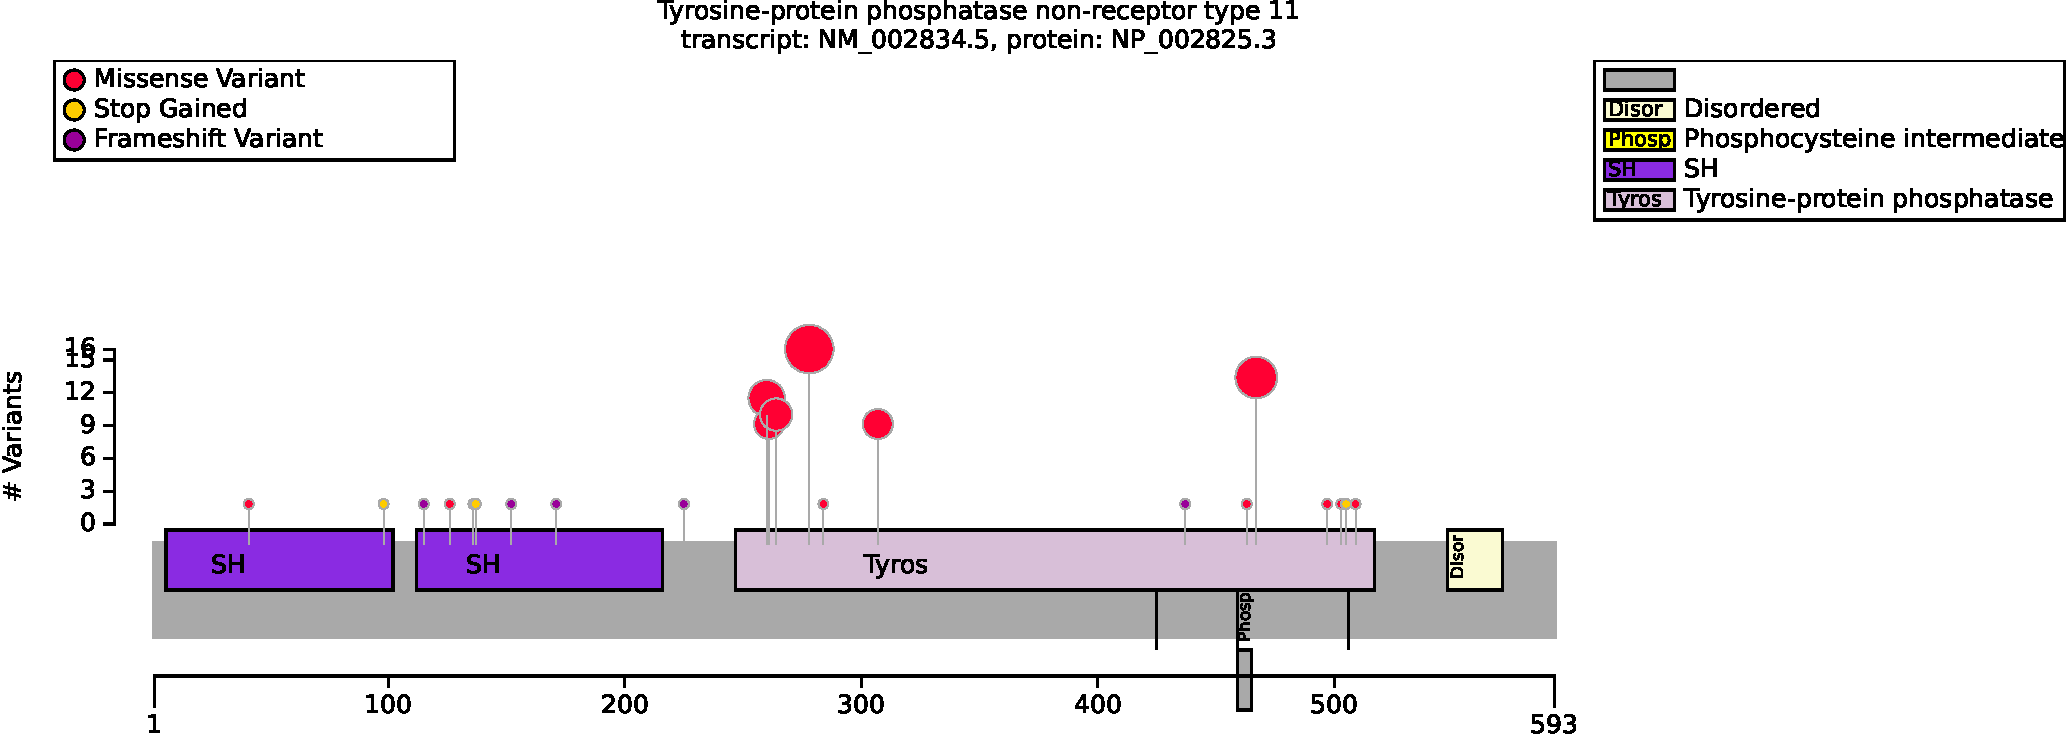
\includegraphics[width=\textwidth]{ img/PTPN11_protein_diagram.pdf} 
\captionsetup{justification=raggedright,singlelinecheck=false}
\caption{Distribution of variants in PTPN11}
\end{subfigure}

\vspace{2em}

\begin{subfigure}[b]{0.95\textwidth}
\centering
\resizebox{\textwidth}{!}{
\begin{tabular}{llllrr}
\toprule
HPO term & Missense & Other & p-value & adj. p-value\\
\midrule
Hypertelorism [HP:0000316] & 37/41 (90\%) & 0/12 (0\%) & $6.82\times 10^{-9}$ & $2.05\times 10^{-8}$\\
Webbed neck [HP:0000465] & 15/20 (75\%) & 0/12 (0\%) & $2.94\times 10^{-5}$ & $4.41\times 10^{-5}$\\
Pulmonic stenosis [HP:0001642] & 18/34 (53\%) & 0/12 (0\%) & 0.001 & 0.001\\
\bottomrule
\end{tabular}
}
\captionsetup{justification=raggedright,singlelinecheck=false}
\caption{Fisher Exact Test performed to compare HPO annotation frequency with respect to Missense and Other. Total of 3 tests were performed.}
\end{subfigure}
\vspace{2em}
\begin{subfigure}[b]{0.95\textwidth}
\centering
\resizebox{\textwidth}{!}{
\begin{tabular}{llllrr}
\toprule
Genotype (A) & Genotype (B) & total tests performed & significant results\\
\midrule
Tyr279Cys & Other & 7 & 0\\
TK domain N term & TK domain C term & 5 & 0\\
FEMALE & MALE & 6 & 0\\
\bottomrule
\end{tabular}
}
\captionsetup{justification=raggedright,singlelinecheck=false}
\caption{Fisher Exact Test performed to compare HPO annotation frequency with respect to genotypes.}
\end{subfigure}

\vspace{2em}

\caption{The cohort comprised 70 individuals (27 females, 33 males, 10 with unknown sex). A total of 69 HPO terms were used to annotate the cohort. Disease diagnoses: LEOPARD syndrome 1 (OMIM:151100) (31 individuals), Noonan syndrome 1 (OMIM:163950) (27 individuals), Metachondromatosis (OMIM:156250) (12 individuals). No previous statistical analysis of correlations with PTPN11 missense variants was identified in the medical literature. A total of 70 unique variant alleles were found in \textit{PTPN11} (transcript: \texttt{NM\_002834.5}, protein id: \texttt{NP\_002825.3}).}
\end{figure}

\begin{figure}[htbp]
\centering
\begin{subfigure}[b]{0.95\textwidth}
\centering
\resizebox{\textwidth}{!}{
\begin{tabular}{llllrr}
\toprule
HPO term & insertion & other & p-value & adj. p-value & ref\\\\
\midrule
Severe global developmental delay [HP:0011344] & 35/41 (85\%) & 0/4 (0\%) & 0.001 & 0.037 & \cite{PMID_38991538} \\
Moderate global developmental delay [HP:0011343] & 6/41 (15\%) & 4/4 (100\%) & 0.001 & 0.037 & \cite{PMID_38991538}\\
\bottomrule
\end{tabular}
}
\captionsetup{justification=raggedright,singlelinecheck=false}
\caption{Fisher Exact Test performed to compare HPO annotation frequency with respect to insertion (n.64\_65insT and three other insertion variants) and other (substition variants). Total of
        53 tests were performed. Note that the results for severe and moderate global developmental delay are symmetrical.}
\end{subfigure}

\vspace{2em}

\begin{subfigure}[b]{0.95\textwidth}
\centering
\resizebox{\textwidth}{!}{
\begin{tabular}{llllrr}
\toprule
Genotype (A) & Genotype (B) & total tests performed & significant results\\
\midrule
n.64\_65insT & other & 53 & 0\\
FEMALE & MALE & 52 & 0\\
\bottomrule
\end{tabular}
}
\captionsetup{justification=raggedright,singlelinecheck=false}
\caption{Fisher Exact Test performed to compare HPO annotation frequency with respect to genotypes.}
\end{subfigure}

\vspace{2em}

\caption{ The cohort comprised 61 individuals (28 females, 33 males). A total of 209 HPO terms were used to annotate the cohort. Disease diagnosis: ReNU syndrome (OMIM:620851). No previous statistical analysis of correlations with PTPN11 missense variants identified in the medical literature. A total of 61 unique variant alleles were found in \textit{RNU4-2} (transcript: \texttt{NR\_003137.3}, protein id: \texttt{}).}
\end{figure}

\begin{figure}[htbp]
\centering
\begin{subfigure}[b]{0.95\textwidth}
\centering
\resizebox{\textwidth}{!}{
\begin{tabular}{llllrr}
\toprule
HPO term & OMIM:268310 & OMIM:616331 & p-value & adj. p-value\\
\midrule
Short stature [HP:0004322] & 29/29 (100\%) & 3/11 (27\%) & $2.15\times 10^{-6}$ & $1.69\times 10^{-4}$\\
Hearing impairment [HP:0000365] & 3/22 (14\%) & 7/7 (100\%) & $7.69\times 10^{-5}$ & 0.003\\
Cleft palate [HP:0000175] & 0/17 (0\%) & 5/8 (62\%) & 0.001 & 0.028\\
Mesomelia [HP:0003027] & 31/31 (100\%) & 10/15 (67\%) & 0.002 & 0.043\\
Orofacial cleft [HP:0000202] & 5/22 (23\%) & 5/5 (100\%) & 0.003 & 0.049\\
\bottomrule
\end{tabular}
}
\captionsetup{justification=raggedright,singlelinecheck=false}
\caption{Fisher Exact Test performed to compare HPO annotation frequency with respect to Robinow syndrome, autosomal recessive (OMIM:268310) and Robinow syndrome, autosomal dominant 2 (OMIM:616331). Total of
        79 tests were performed. }
\end{subfigure}
\vspace{2em}
\caption{The cohort comprised 48 individuals (10 females, 14 males, 24 with unknown sex). A total of 103 HPO terms were used to annotate the cohort. Disease diagnoses: Robinow syndrome, autosomal recessive (OMIM:268310) (32 individuals), Robinow syndrome, autosomal dominant 2 (OMIM:616331) (16 individuals). Robinow syndrome is a skeletal dysplasia characterized by dysmorphic facial features, short-limbed dwarfism, vertebral segmentation, and genital hypoplasia.}
\end{figure}

\begin{figure}[htbp]
\centering
\begin{subfigure}[b]{0.95\textwidth}
\centering
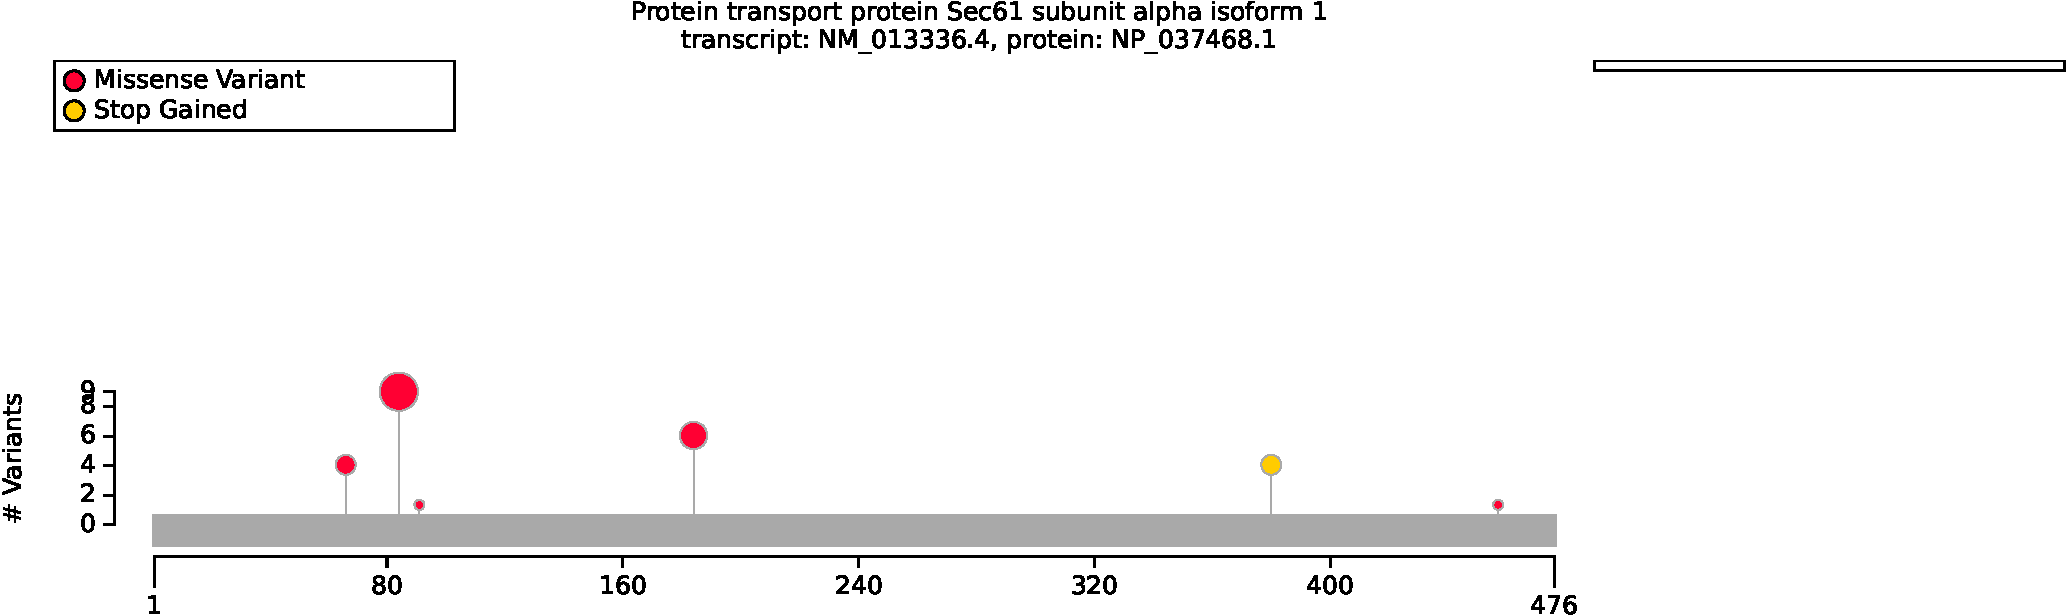
\includegraphics[width=\textwidth]{img/SEC61A1_protein_diagram.pdf} 
\captionsetup{justification=raggedright,singlelinecheck=false}
\caption{Distribution of variants in SEC61A1}
\end{subfigure}

\vspace{2em}

\begin{subfigure}[b]{0.95\textwidth}
\centering
\resizebox{\textwidth}{!}{
\begin{tabular}{llllrr}
\toprule
HPO term & p.Val85Asp & Other variant & p-value & adj. p-value\\
\midrule
Recurrent lower respiratory tract infections [HP:0002783] & 6/6 (100\%) & 0/5 (0\%) & 0.002 & 0.039\\
\bottomrule
\end{tabular}
}
\captionsetup{justification=raggedright,singlelinecheck=false}
\caption{Fisher Exact Test performed to compare HPO annotation frequency with respect to p.Val85Asp and Other variant. Total of
        18 tests were performed.}
\end{subfigure}
\vspace{2em}
\begin{subfigure}[b]{0.95\textwidth}
\centering
\resizebox{\textwidth}{!}{
\begin{tabular}{llllrr}
\toprule
Genotype (A) & Genotype (B) & total tests performed & significant results\\
\midrule
FEMALE & MALE & 24 & 0\\
\bottomrule
\end{tabular}
}
\captionsetup{justification=raggedright,singlelinecheck=false}
\caption{Fisher Exact Test performed to compare HPO annotation frequency with respect to genotypes.}
\end{subfigure}

\vspace{2em}

\caption{The cohort comprised 19 individuals (8 females, 11 males). 1 of these individuals were reported to be deceased. 
A total of 76 HPO terms were used to annotate the cohort. Disease diagnoses: Immunodeficiency, common variable, 15 (OMIM:620670) (11 individuals), 
Tubulointerstitial kidney disease, autosomal dominant, 5 (OMIM:617056) (7 individuals), Neutropenia, severe congenital, 11, autosomal dominant (OMIM:620674) 
(1 individuals). The origin of clinical diversity in patients with SEC61A1 mutation is currently unclear. 
With our present patient set, a particular phenotype cannot be predicted on the basis of location or nature of the mutation \cite{PMID_32325141}. 
A total of 19 unique variant alleles were found in \textit{SEC61A1} (transcript: \texttt{NM\_013336.4}, protein id: \texttt{NP\_037468.1}).}
\end{figure}

\begin{figure}[htbp]
\section*{SF3B4}
\centering
\begin{subfigure}[b]{0.95\textwidth}
\centering
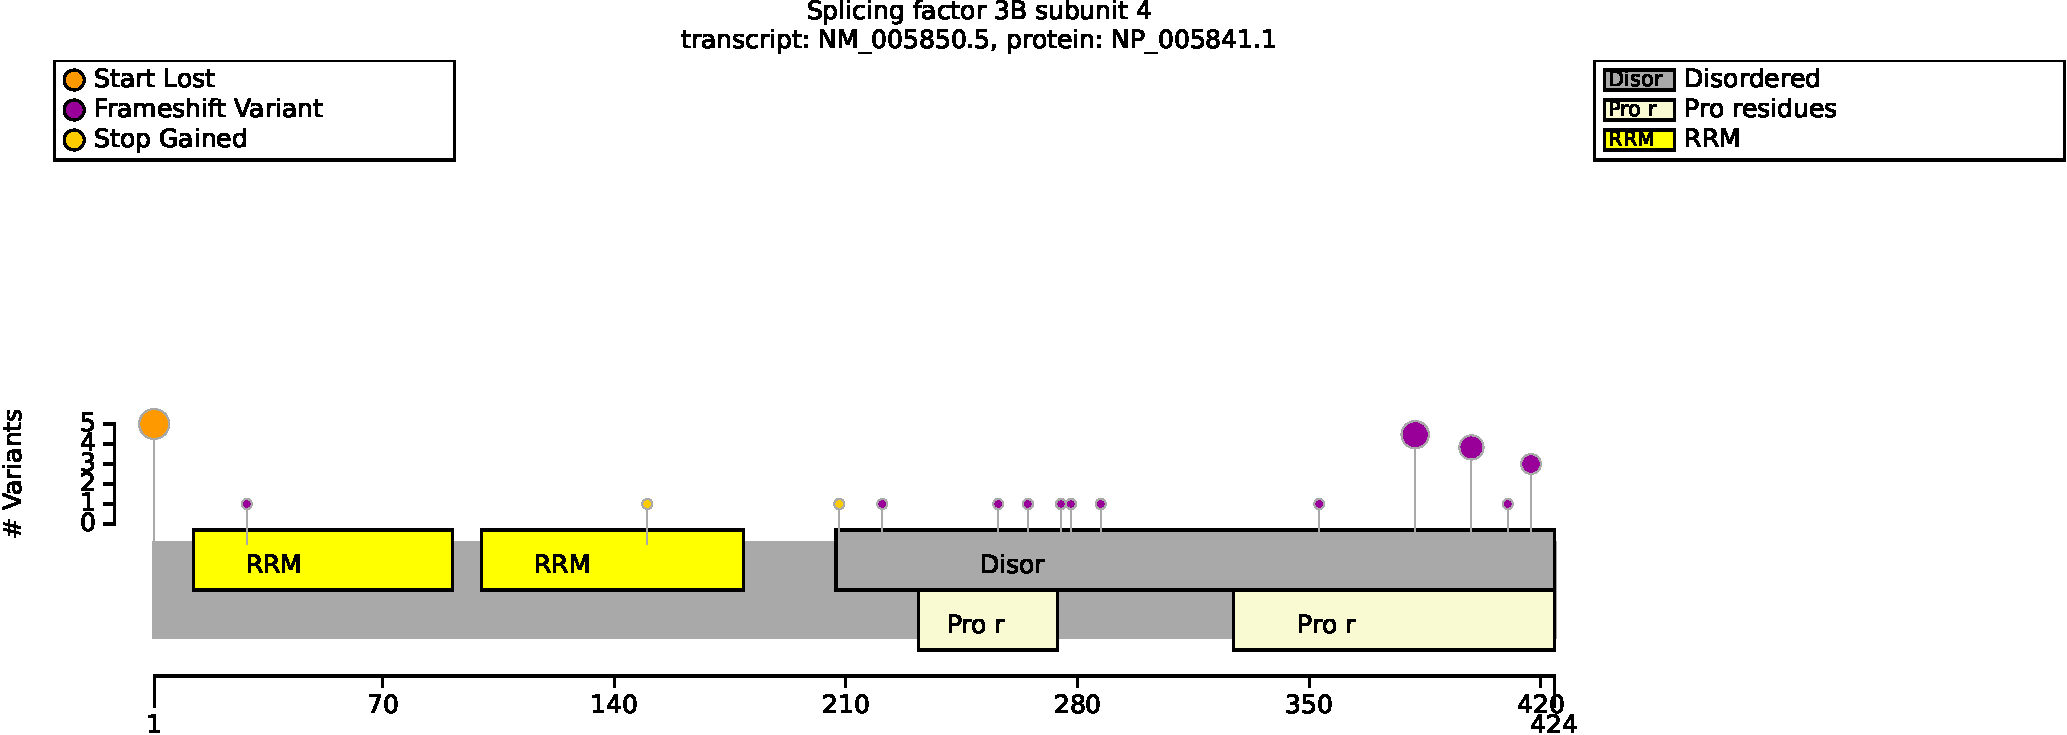
\includegraphics[width=\textwidth]{ img/SF3B4_protein_diagram.pdf} 
\captionsetup{justification=raggedright,singlelinecheck=false}
\caption{Distribution of variants in SF3B4}
\end{subfigure}

\vspace{2em}

\begin{subfigure}[b]{0.95\textwidth}
\centering
\resizebox{\textwidth}{!}{
\begin{tabular}{llllrr}
\toprule
Genotype (A) & Genotype (B) & total tests performed & significant results\\
\midrule
p.Met1? & Other & 46 & 0\\
FEMALE & MALE & 46 & 0\\
\bottomrule
\end{tabular}
}
\captionsetup{justification=raggedright,singlelinecheck=false}
\caption{Fisher Exact Test performed to compare HPO annotation frequency with respect to genotypes.}
\end{subfigure}

\vspace{2em}

\caption{The cohort comprised 26 individuals (18 females, 8 males). A total of 41 HPO terms were used to annotate the cohort. Disease diagnosis: Acrofacial dysostosis 1, Nager type (OMIM:154400). 
In one published analysis, it was stated that ``although no significant genotype–phenotype association was found, it is notable that patients with frameshift SF3B4 variants and predicted to lead to nonsense-mediated RNA 
decay (NMD) of the transcripts tended to have a more severe clinical manifestation''. The authors did not correct for multiple testing and did not find nominally significant associations \cite{PMID_35331022}.
No significant correlation found in our study. A total of 18 unique variant alleles were found in \textit{SF3B4} (transcript: \texttt{NM\_005850.5}, protein id: \texttt{NP\_005841.1}).}
\end{figure}




\begin{figure}[htbp]
    \section*{SLC45A2}
\centering
\begin{subfigure}[b]{0.95\textwidth}
\centering
\resizebox{\textwidth}{!}{
\begin{tabular}{llllrr}
\toprule
Genotype (A) & Genotype (B) & total tests performed & significant results\\
\midrule
missense/missense OR missense/other & other/other & 24 & 0\\
FEMALE & MALE & 25 & 0\\
\bottomrule
\end{tabular}
}
\captionsetup{justification=raggedright,singlelinecheck=false}
\caption{Fisher Exact Test performed to compare HPO annotation frequency with respect to genotypes. }
\end{subfigure}

\vspace{2em}

\caption{The cohort comprised 30 individuals (17 females, 13 males). A total of 16 HPO terms were used to annotate the cohort. Disease diagnosis: Albinism, oculocutaneous, type IV (OMIM:606574). No significant association identified. A total of 28 unique variant alleles were found in \textit{SLC45A2} (transcript: \texttt{NM\_016180.5}, protein id: \texttt{NP\_057264.4}).}
\end{figure}




\begin{figure}[htbp]
    \section*{SMAD2}
\centering
\begin{subfigure}[b]{0.95\textwidth}
\centering
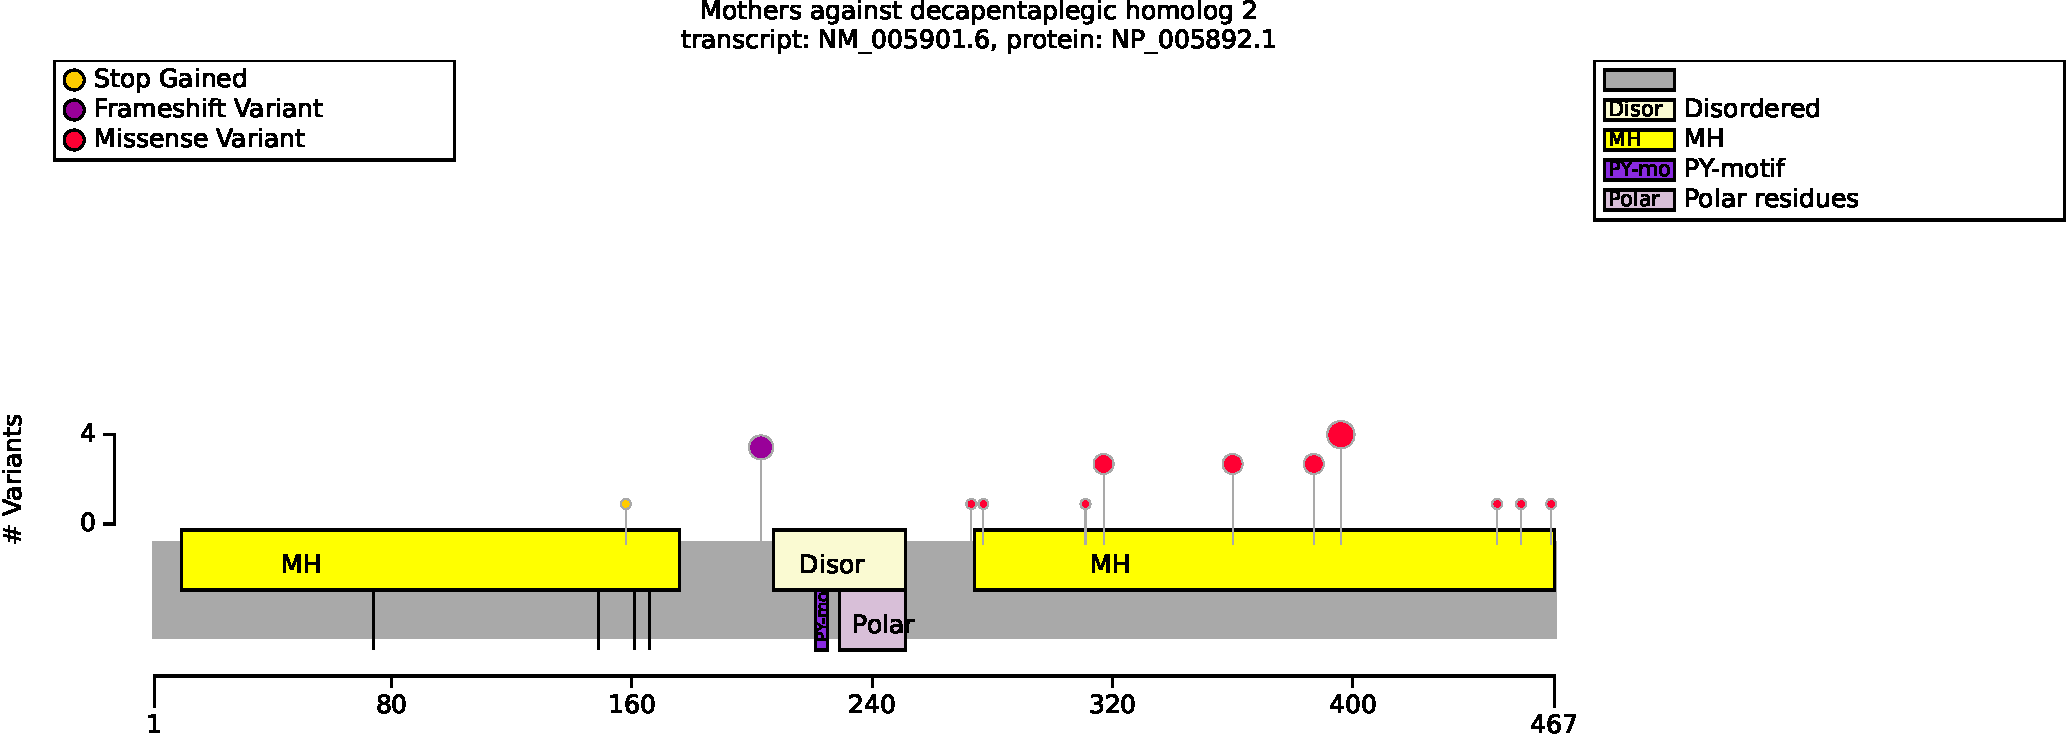
\includegraphics[width=\textwidth]{ img/SMAD2_protein_diagram.pdf} 
\captionsetup{justification=raggedright,singlelinecheck=false}
\caption{Distribution of variants in SMAD2}
\end{subfigure}

\vspace{2em}

\begin{subfigure}[b]{0.95\textwidth}
\centering
\resizebox{\textwidth}{!}{
\begin{tabular}{llllrr}
\toprule
Genotype (A) & Genotype (B) & total tests performed & significant results\\
\midrule
Ser397Tyr & Other & 19 & 0\\
N Term & Other & 19 & 0\\
FEMALE & MALE & 19 & 0\\
\bottomrule
\end{tabular}
}
\captionsetup{justification=raggedright,singlelinecheck=false}
\caption{Fisher Exact Test performed to compare HPO annotation frequency with respect to genotypes.}
\end{subfigure}

\vspace{2em}

\caption{ The cohort comprised 23 individuals (13 females, 8 males, 2 with unknown sex). A total of 89 HPO terms were used to annotate the cohort. Disease diagnoses: Loeys-Dietz syndrome 6 (OMIM:619656) (18 individuals), Congenital heart defects, multiple types, 8, with or without heterotaxy (OMIM:619657) (5 individuals). We were not able to identify published results suggesting correlations with specific SMAD2 residues or variant categories. A total of 23 unique variant alleles were found in \textit{SMAD2} (transcript: \texttt{NM\_005901.6}, protein id: \texttt{NP\_005892.1}).}
\end{figure}

\section*{SMAD3}

\begin{figure}[htbp]
\centering
\begin{subfigure}[b]{0.95\textwidth}
\centering
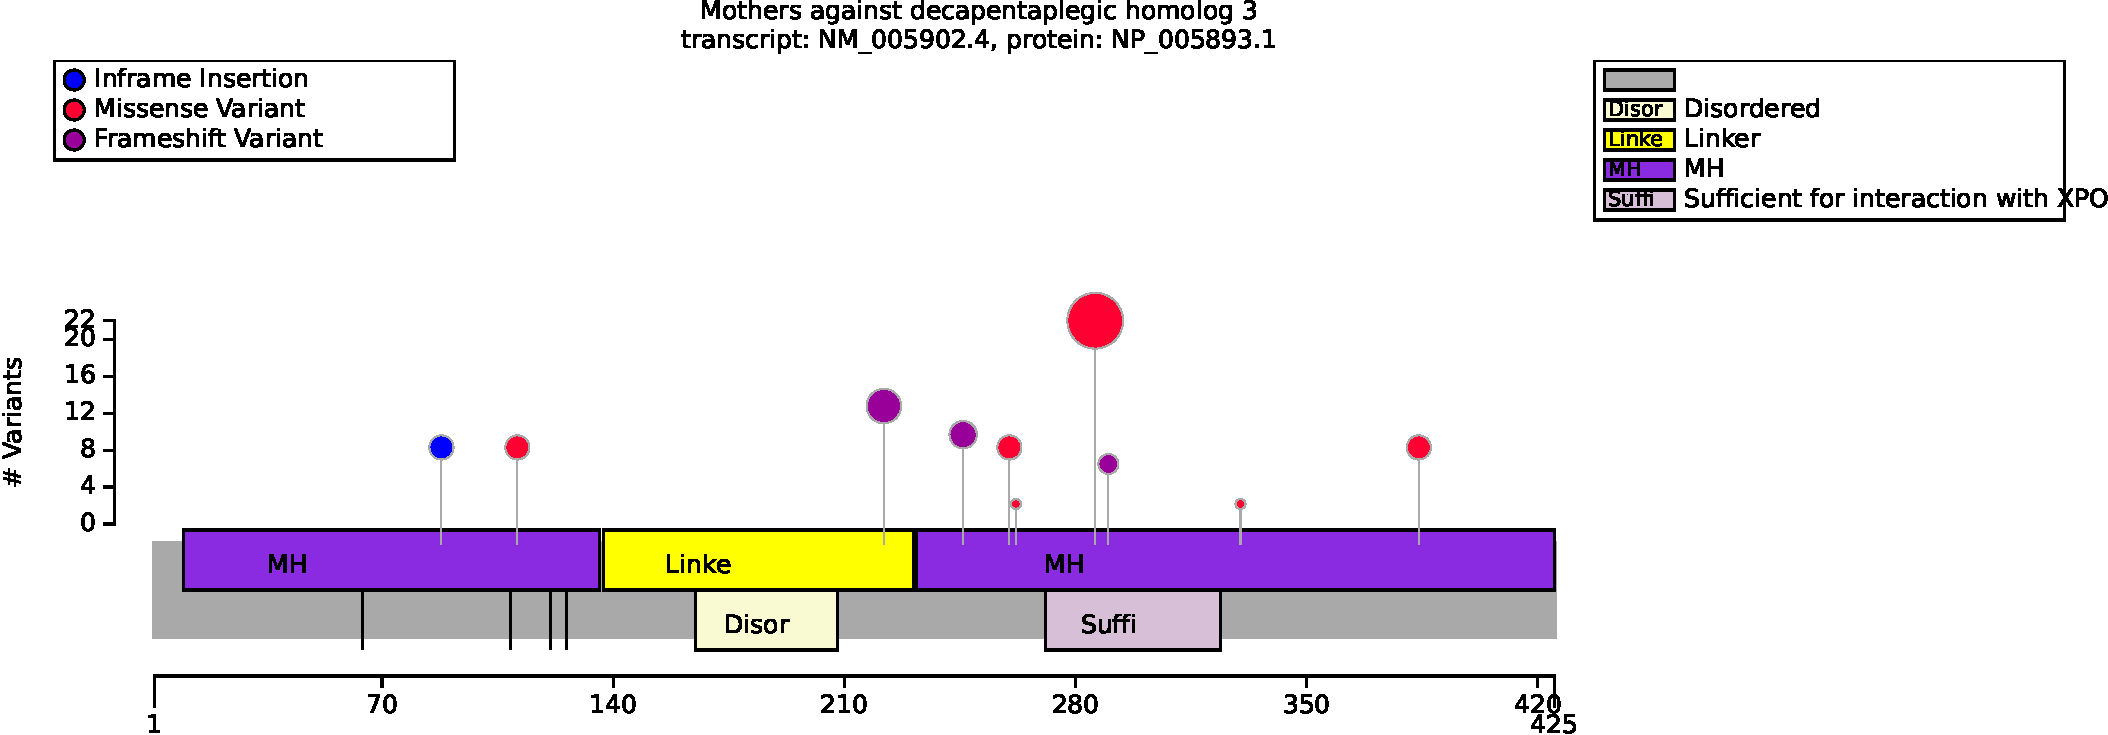
\includegraphics[width=\textwidth]{ img/SMAD3_protein_diagram.pdf} 
\captionsetup{justification=raggedright,singlelinecheck=false}
\caption{Distribution of variants in SMAD3}
\end{subfigure}

\vspace{2em}

\begin{subfigure}[b]{0.95\textwidth}
\centering
\resizebox{\textwidth}{!}{
\begin{tabular}{llllrr}
\toprule
HPO term & p.Arg287Trp & Other & p-value & adj. p-value\\
\midrule
Osteoarthritis [HP:0002758] & 19/19 (100\%) & 7/19 (37\%) & $3.72\times 10^{-5}$ & $8.56\times 10^{-4}$\\
\bottomrule
\end{tabular}
}
\captionsetup{justification=raggedright,singlelinecheck=false}
\caption{Fisher Exact Test performed to compare HPO annotation frequency with respect to p.Arg287Trp and Other. Total of
        23 tests were performed.}
\end{subfigure}
\vspace{2em}
\begin{subfigure}[b]{0.95\textwidth}
\centering
\resizebox{\textwidth}{!}{
\begin{tabular}{llllrr}
\toprule
Genotype (A) & Genotype (B) & total tests performed & significant results\\
\midrule
missense & other & 24 & 0\\
FEMALE & MALE & 22 & 0\\
\bottomrule
\end{tabular}
}
\captionsetup{justification=raggedright,singlelinecheck=false}
\caption{Fisher Exact Test performed to compare HPO annotation frequency with respect to genotypes. }
\end{subfigure}

\vspace{2em}

\caption{ The cohort comprised 49 individuals (22 females, 27 males). 
A total of 30 HPO terms were used to annotate the cohort. Disease diagnosis: Loeys-Dietz syndrome 3 
(OMIM:613795). There was no evidence of a correlation between missense variants and specific 
phenotypic abnormalities. In contrast, there was a statistically significant correlation with 
Arg287Trp and Osteoarthritis. The residue Arg287 is located in the Mad homology 2 (MH2) domain in a 
region that mediates interaction with exportin 4 \cite{PMID_16449645}. Chesneau et al stated that there is an absence of correlation between the SMAD3 variant type and the occurrence of aortic phenotypes \cite{PMID_32154675}.
To the best of our knowledge an association between Arg287Trp and Osteoarthritis has not been previously noted.
A total of 49 unique variant alleles were found in \textit{SMAD3} (transcript: \texttt{NM\_005902.4}, protein id: \texttt{NP\_005893.1}).}
\end{figure}


\begin{figure}[htbp]
    \section*{SMARCB1}
\centering
\begin{subfigure}[b]{0.75\textwidth}
\centering
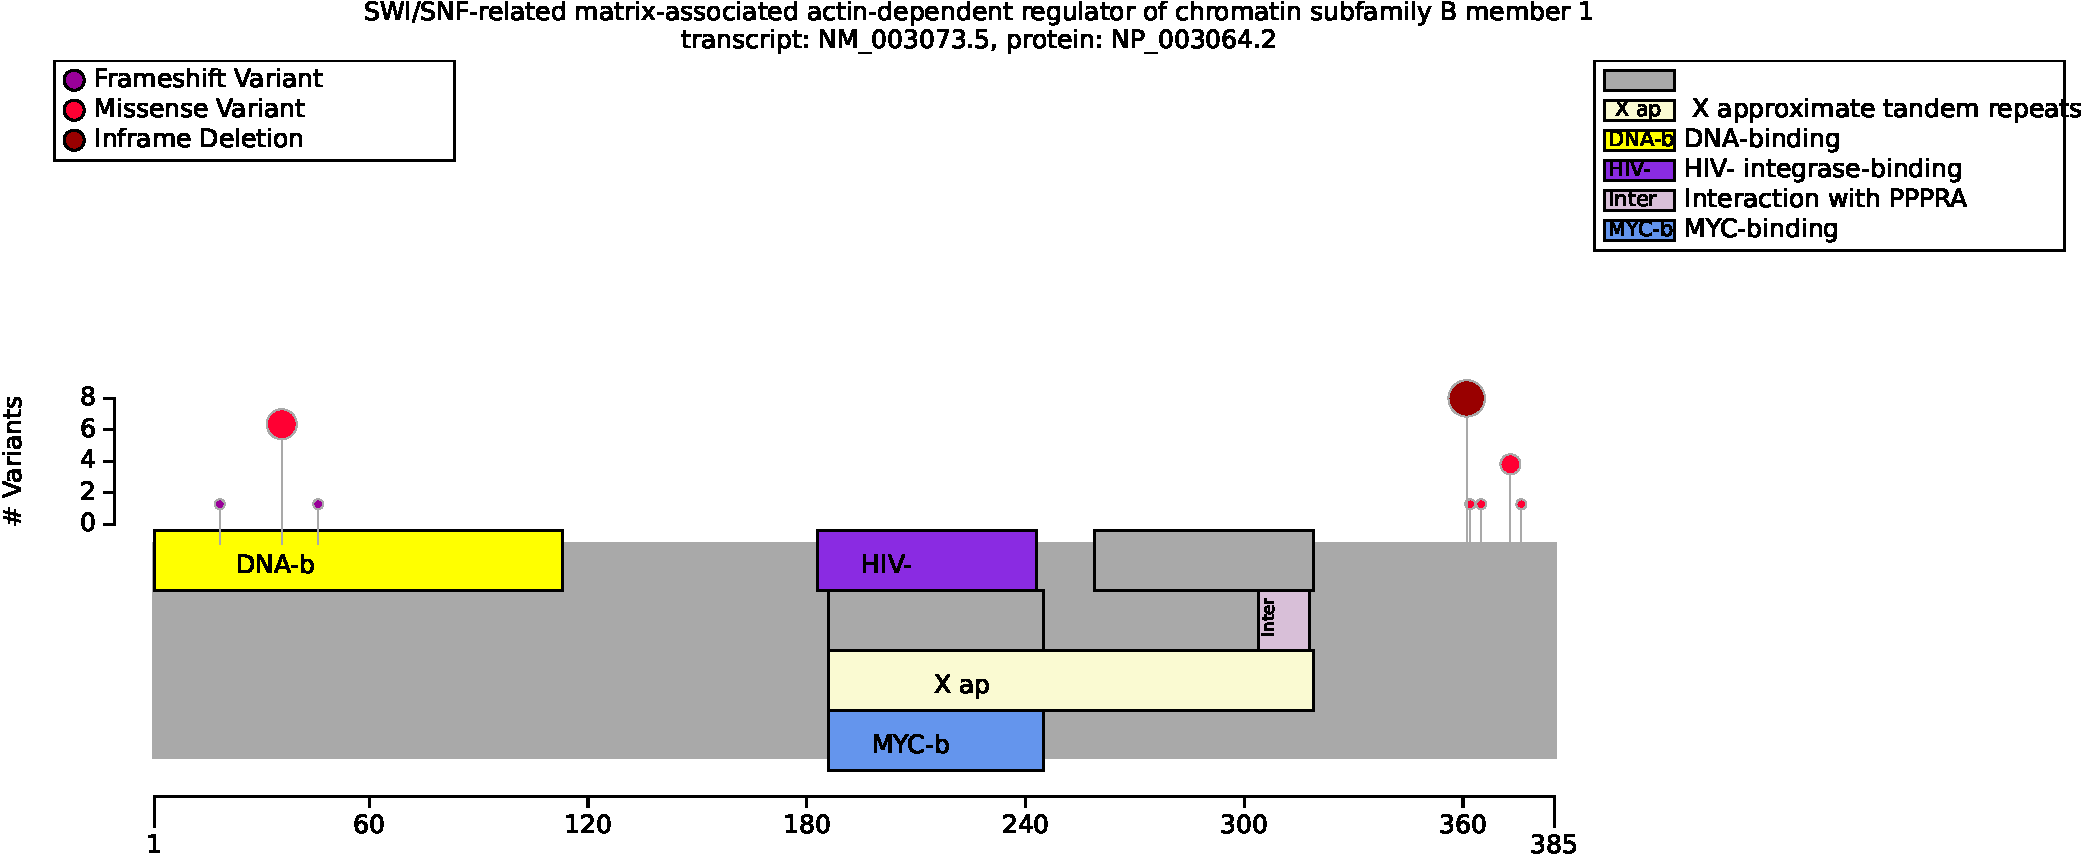
\includegraphics[width=\textwidth]{ img/SMARCB1_protein_diagram.pdf} 
\captionsetup{justification=raggedright,singlelinecheck=false}
\caption{Distribution of variants in SMARCB1}
\end{subfigure}

\begin{subfigure}[b]{0.95\textwidth}
\centering
\resizebox{\textwidth}{!}{
\begin{tabular}{llllrr}
\toprule
HPO term & Structural variant & Other & p-value & adj. p-value\\
\midrule
Neoplasm by histology [HP:0011792] & 11/11 (100\%) & 4/21 (19\%) & $1.06\times 10^{-5}$ & $1.01\times 10^{-4}$\\
Embryonal neoplasm [HP:0002898] & 8/8 (100\%) & 2/19 (11\%) & $2.03\times 10^{-5}$ & $1.01\times 10^{-4}$\\
Atypical teratoid/rhabdoid tumor [HP:0034401] & 8/9 (89\%) & 2/19 (11\%) & $1.19\times 10^{-4}$ & $3.96\times 10^{-4}$\\
Rhabdoid tumor [HP:0034557] & 4/4 (100\%) & 2/19 (11\%) & 0.002 & 0.004\\
Neoplasm by anatomical site [HP:0011793] & 3/3 (100\%) & 3/20 (15\%) & 0.011 & 0.019\\
Neuroepithelial neoplasm [HP:0030063] & 2/2 (100\%) & 0/17 (0\%) & 0.006 & 0.012\\
Neoplasm of the nervous system [HP:0004375] & 2/2 (100\%) & 2/19 (11\%) & 0.029 & 0.041\\
\bottomrule
\end{tabular}
}
\captionsetup{justification=raggedright,singlelinecheck=false}
\caption{Fisher Exact Test. Total of 10 tests were performed. }
\end{subfigure}
\vspace{1em}
\begin{subfigure}[b]{0.75\textwidth}
\centering
\resizebox{\textwidth}{!}{
\begin{tabular}{llllrr}
\toprule
Genotype (A) & Genotype (B) & total tests performed & significant results\\
\midrule
Lys364del & Other & 36 & 0\\
DNA binding & Other & 33 & 0\\
\bottomrule
\end{tabular}
}
\captionsetup{justification=raggedright,singlelinecheck=false}
\caption{Fisher Exact Test performed to compare HPO annotation frequency with respect to genotypes. }
\end{subfigure}

\caption{The cohort comprised 32 individuals (12 females, 8 males, 12 with unknown sex). 9 of these individuals were 
reported to be deceased. A total of 110 HPO terms were used to annotate the cohort. Disease diagnoses: 
Coffin-Siris syndrome 3 (OMIM:614608) (18 individuals), Rhabdoid tumor predisposition syndrome 1 (OMIM:609322) 
(14 individuals). Our analysis of SMARCB1 included variants associated with Coffin-Siris syndrome 3 (OMIM:614608).
A total of 32 unique variant alleles were found in \textit{SMARCB1} (transcript: \texttt{NM\_003073.5}, 
protein id: \texttt{NP\_003064.2}). Presumably the result of embryonal neoplasm being signficantly associated with structural variants relates to a 
different distribution of variants in rhabdoid tumor predisposition syndrome-1 than in Coffin-Siris syndrome 3.
A published analysis of GPCs in Coffin-Siris syndrome did not present a statistical analysis and did not note the current association \cite{PMID_25168959}.}
\end{figure}


\begin{figure}[htbp]
\section*{SON}
\centering
\begin{subfigure}[b]{0.95\textwidth}
\centering
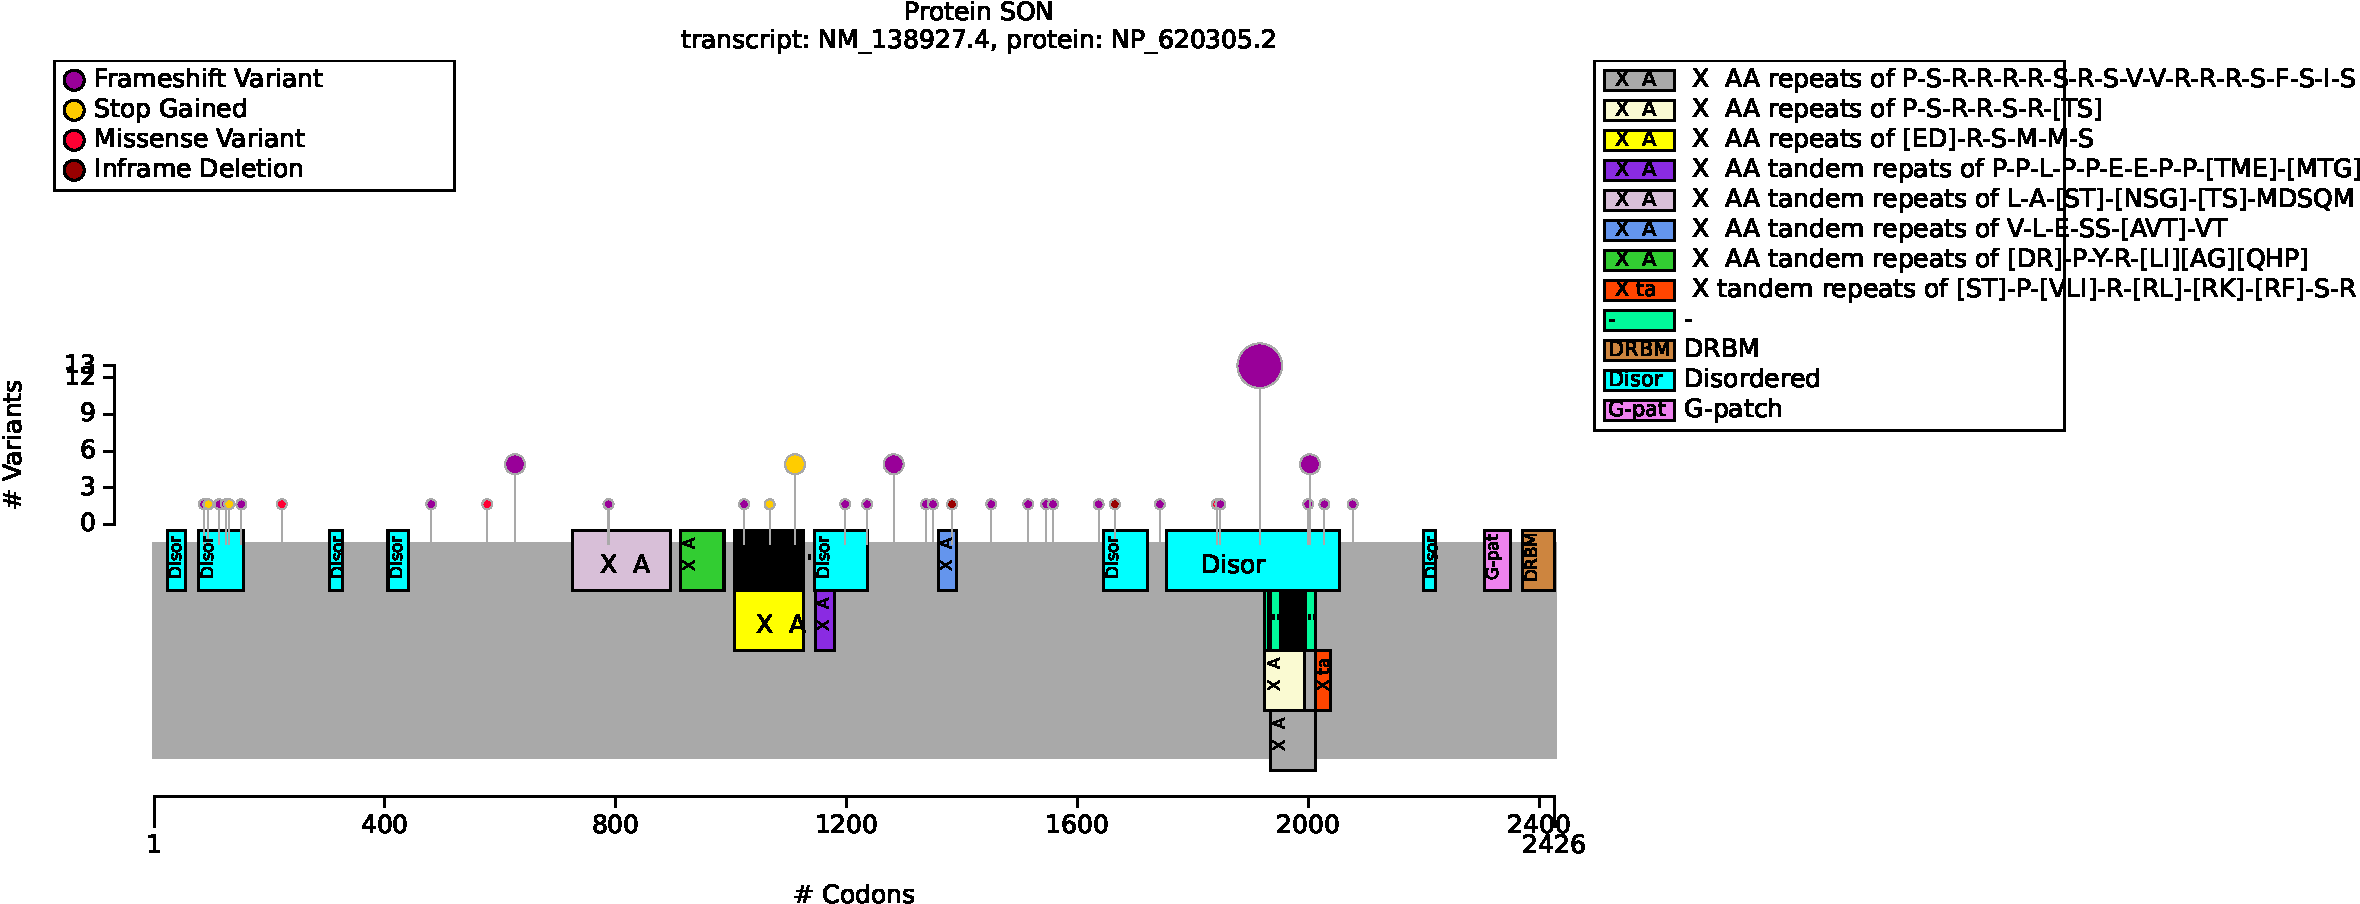
\includegraphics[width=\textwidth]{img/SON_protein_diagram.pdf} 
\captionsetup{justification=raggedright,singlelinecheck=false}
\caption{Distribution of variants in SON}
\end{subfigure}

\vspace{2em}

\begin{subfigure}[b]{0.95\textwidth}
\centering
\resizebox{\textwidth}{!}{
\begin{tabular}{llllrr}
\toprule
Genotype (A) & Genotype (B) & total tests performed & significant results\\
\midrule
missense & Other & 48 & 0\\
c.5753\_5756del & Other & 51 & 0\\
FEMALE & MALE & 51 & 0\\
\bottomrule
\end{tabular}
}
\captionsetup{justification=raggedright,singlelinecheck=false}
\caption{Fisher Exact Test performed to compare HPO annotation frequency with respect to genotypes.}
\end{subfigure}

\vspace{2em}

\caption{ The cohort comprised 52 individuals (26 females, 26 males). A total of 47 HPO terms were used to annotate the cohort. 
Disease diagnosis: ZTTK SYNDROME (OMIM:617140). Dingemans et al (2020) suggested a different pathomechanism for missense variants, 
but our cohort only contains 3 individuals with missense variants, so there is no statistical power \cite{PMID_34521999}. 
A total of 35 unique variant alleles were found in \textit{SON} (transcript: \texttt{NM\_138927.4}, protein id: \texttt{NP\_620305.2}).}
\end{figure}

\begin{figure}[htbp]
\section*{ TBCK}
\centering
\begin{subfigure}[b]{0.95\textwidth}
\centering
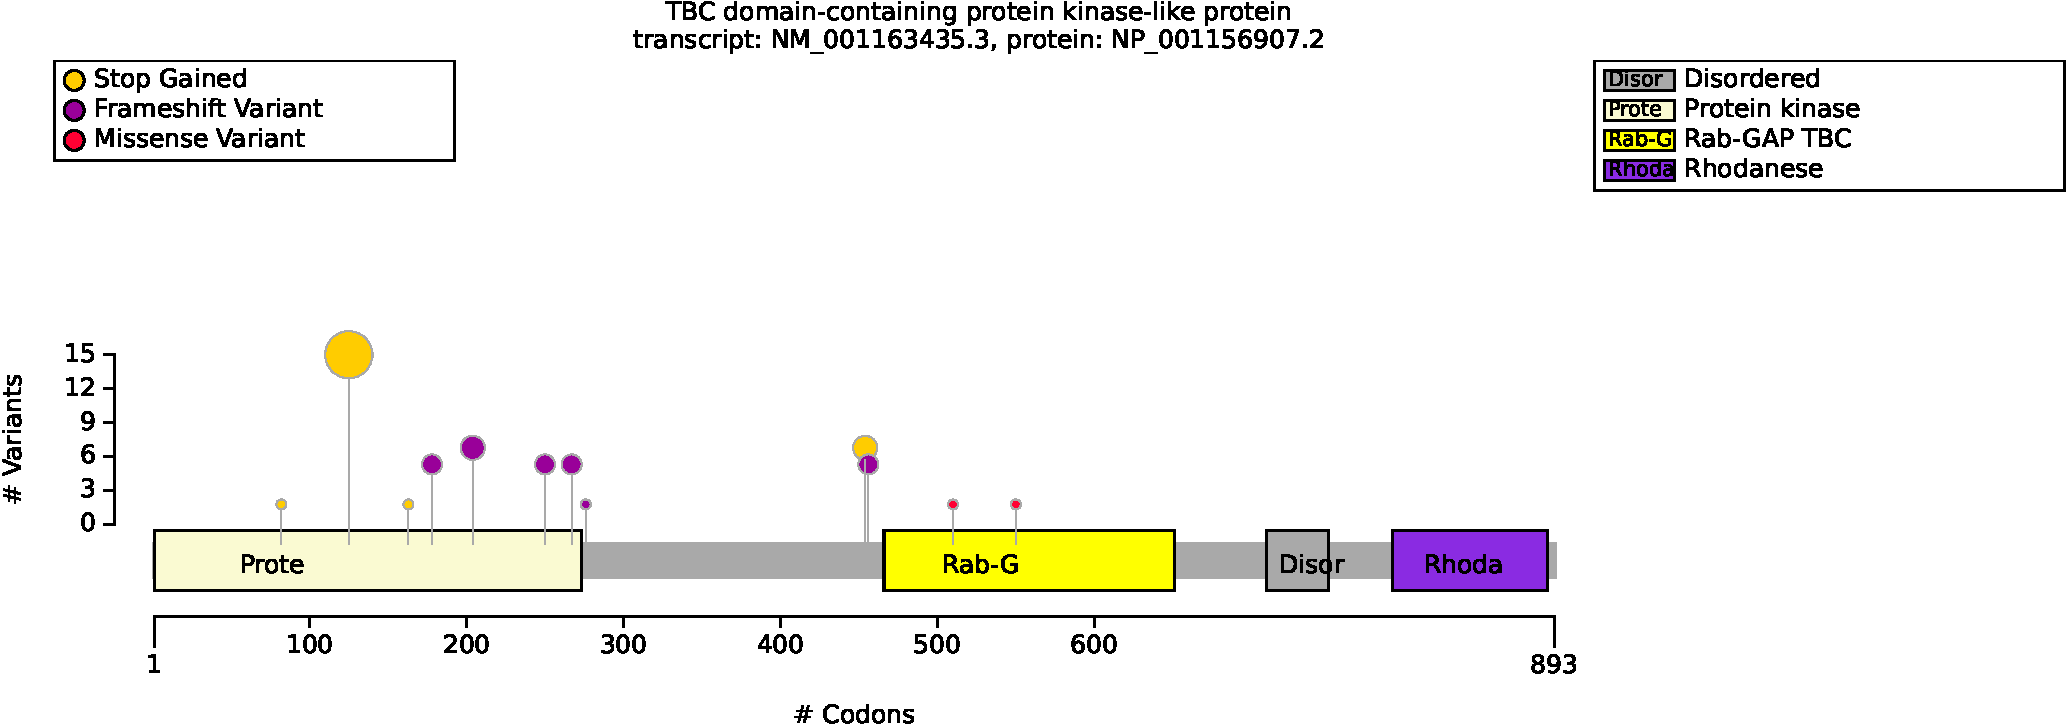
\includegraphics[width=\textwidth]{ img/TBCK_protein_diagram.pdf} 
\captionsetup{justification=raggedright,singlelinecheck=false}
\caption{Distribution of variants in TBCK}
\end{subfigure}

\vspace{2em}

\begin{subfigure}[b]{0.95\textwidth}
\centering
\resizebox{\textwidth}{!}{
\begin{tabular}{llllrr}
\toprule
HPO term & R126*/R126* & R126*/other OR other/other & p-value & adj. p-value\\
\midrule
Macroglossia [HP:0000158] & 11/12 (92\%) & 3/22 (14\%) & $1.34\times 10^{-5}$ & $4.30\times 10^{-4}$\\
Developmental regression [HP:0002376] & 9/12 (75\%) & 2/22 (9\%) & $1.83\times 10^{-4}$ & 0.003\\
\bottomrule
\end{tabular}
}
\captionsetup{justification=raggedright,singlelinecheck=false}
\caption{Fisher Exact Test performed to compare HPO annotation frequency with respect to R126*/R126* and R126*/other OR other/other. Total of
        32 tests were performed.}
\end{subfigure}
\vspace{2em}
\begin{subfigure}[b]{0.95\textwidth}
\centering
\resizebox{\textwidth}{!}{
\begin{tabular}{llllrr}
\toprule
Genotype (A) & Genotype (B) & total tests performed & significant results\\
\midrule
missense/missense OR missense/other & other/other & 30 & 0\\
FEMALE & MALE & 32 & 0\\
\bottomrule
\end{tabular}
}
\captionsetup{justification=raggedright,singlelinecheck=false}
\caption{Fisher Exact Test performed to compare HPO annotation frequency with respect to genotypes.}
\end{subfigure}

\vspace{2em}

\caption{ The cohort comprised 41 individuals (17 females, 24 males). 3 of these individuals were reported to be deceased. A total of 97 HPO terms were used to annotate the cohort. 
Disease diagnosis: Hypotonia, infantile, with psychomotor retardation and characteristic facies 3 (OMIM:616900). 
Durham et al (2023) stated that several studies have touched on a genotype-phenotype correlation of TBCK syndrome; however, more data are required for statistically significant conclusions \cite{PMID_37455236}. 
A total of 18 unique variant alleles were found in \textit{TBCK} (transcript: \texttt{NM\_001163435.3}, protein id: \texttt{NP\_001156907.2}).}
\end{figure}

\begin{figure}[htbp]
\section*{ TGFB2}
\centering
\begin{subfigure}[b]{0.95\textwidth}
\centering
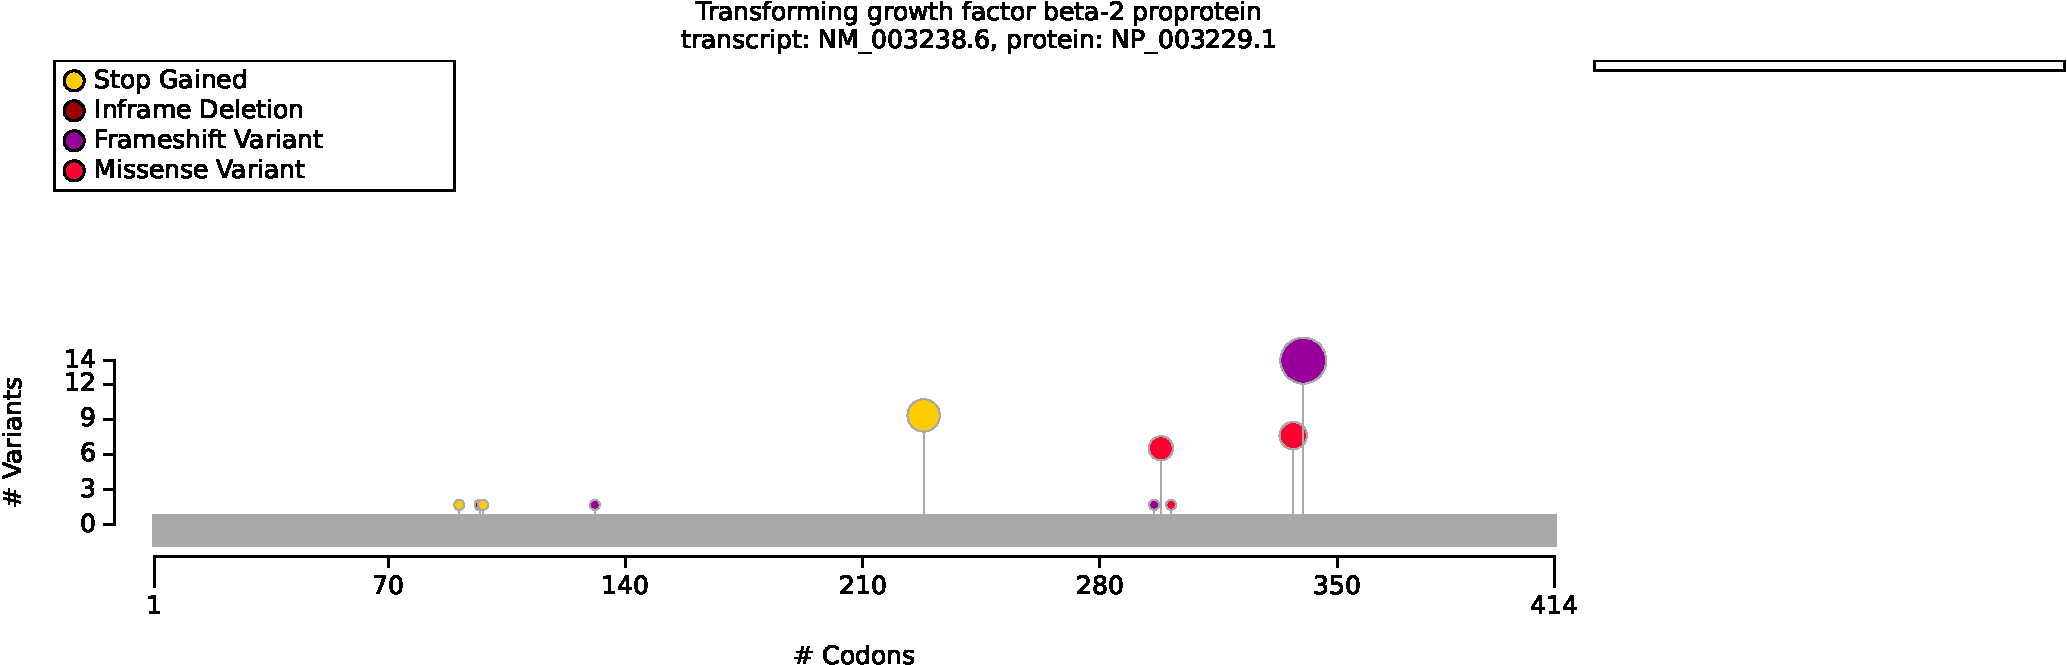
\includegraphics[width=\textwidth]{ img/TGFB2_protein_diagram.pdf} 
\captionsetup{justification=raggedright,singlelinecheck=false}
\caption{Distribution of variants in TGFB2}
\end{subfigure}

\vspace{2em}

\begin{subfigure}[b]{0.95\textwidth}
\centering
\resizebox{\textwidth}{!}{
\begin{tabular}{llllrr}
\toprule
Genotype (A) & Genotype (B) & total tests performed & significant results\\
\midrule
missense & other & 37 & 0\\
FEMALE & MALE & 38 & 0\\
\bottomrule
\end{tabular}
}
\captionsetup{justification=raggedright,singlelinecheck=false}
\caption{Fisher Exact Test performed to compare HPO annotation frequency with respect to genotypes. }
\end{subfigure}

\vspace{2em}

\caption{ The cohort comprised 36 individuals (10 females, 26 males). 1 of these individuals were reported to be deceased. A total of 68 HPO terms were used to annotate the cohort. Disease diagnosis: Loeys-Dietz syndrome 4 (OMIM:614816). No significant association found. A total of 12 unique variant alleles were found in \textit{TGFB2} (transcript: \texttt{NM\_003238.6}, protein id: \texttt{NP\_003229.1}).}
\end{figure}

\begin{figure}[htbp]
\section*{ TGFB3}
\centering
\begin{subfigure}[b]{0.95\textwidth}
\centering
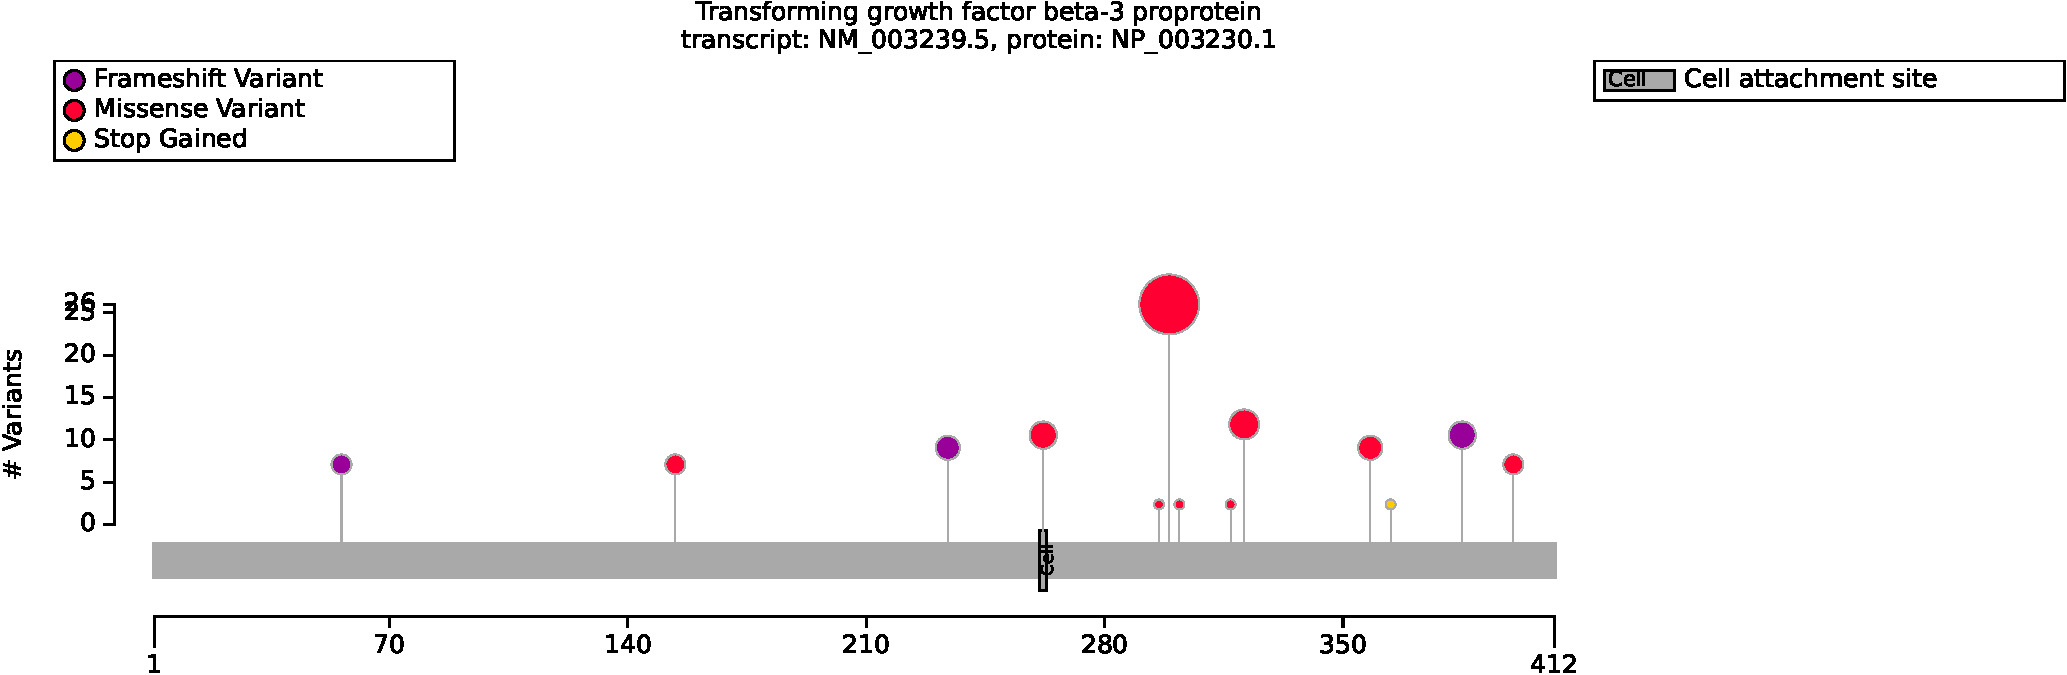
\includegraphics[width=\textwidth]{ img/TGFB3_protein_diagram.pdf} 
\captionsetup{justification=raggedright,singlelinecheck=false}
\caption{Distribution of variants in TGFB3}
\end{subfigure}

\vspace{2em}

\begin{subfigure}[b]{0.95\textwidth}
\centering
\resizebox{\textwidth}{!}{
\begin{tabular}{llllrr}
\toprule
Genotype (A) & Genotype (B) & total tests performed & significant results\\
\midrule
Missense & Other & 12 & 0\\
Asp263His & Other & 10 & 0\\
FEMALE & MALE & 13 & 0\\
\bottomrule
\end{tabular}
}
\captionsetup{justification=raggedright,singlelinecheck=false}
\caption{             Fisher Exact Test performed to compare HPO annotation frequency with respect to genotypes. }
\end{subfigure}

\vspace{2em}

\caption{ The cohort comprised 75 individuals (34 females, 41 males). 7 of these individuals were reported to be deceased. A total of 73 HPO terms were used to annotate the cohort. Disease diagnosis: Loeys-Dietz syndrome 5 (OMIM:615582). No significant correlations identified. A total of 75 unique variant alleles were found in \textit{TGFB3} (transcript: \texttt{NM\_003239.5}, protein id: \texttt{NP\_003230.1}).}
\end{figure}

\begin{figure}[htbp]
\section*{ TGFBR2}
\centering
\begin{subfigure}[b]{0.95\textwidth}
\centering
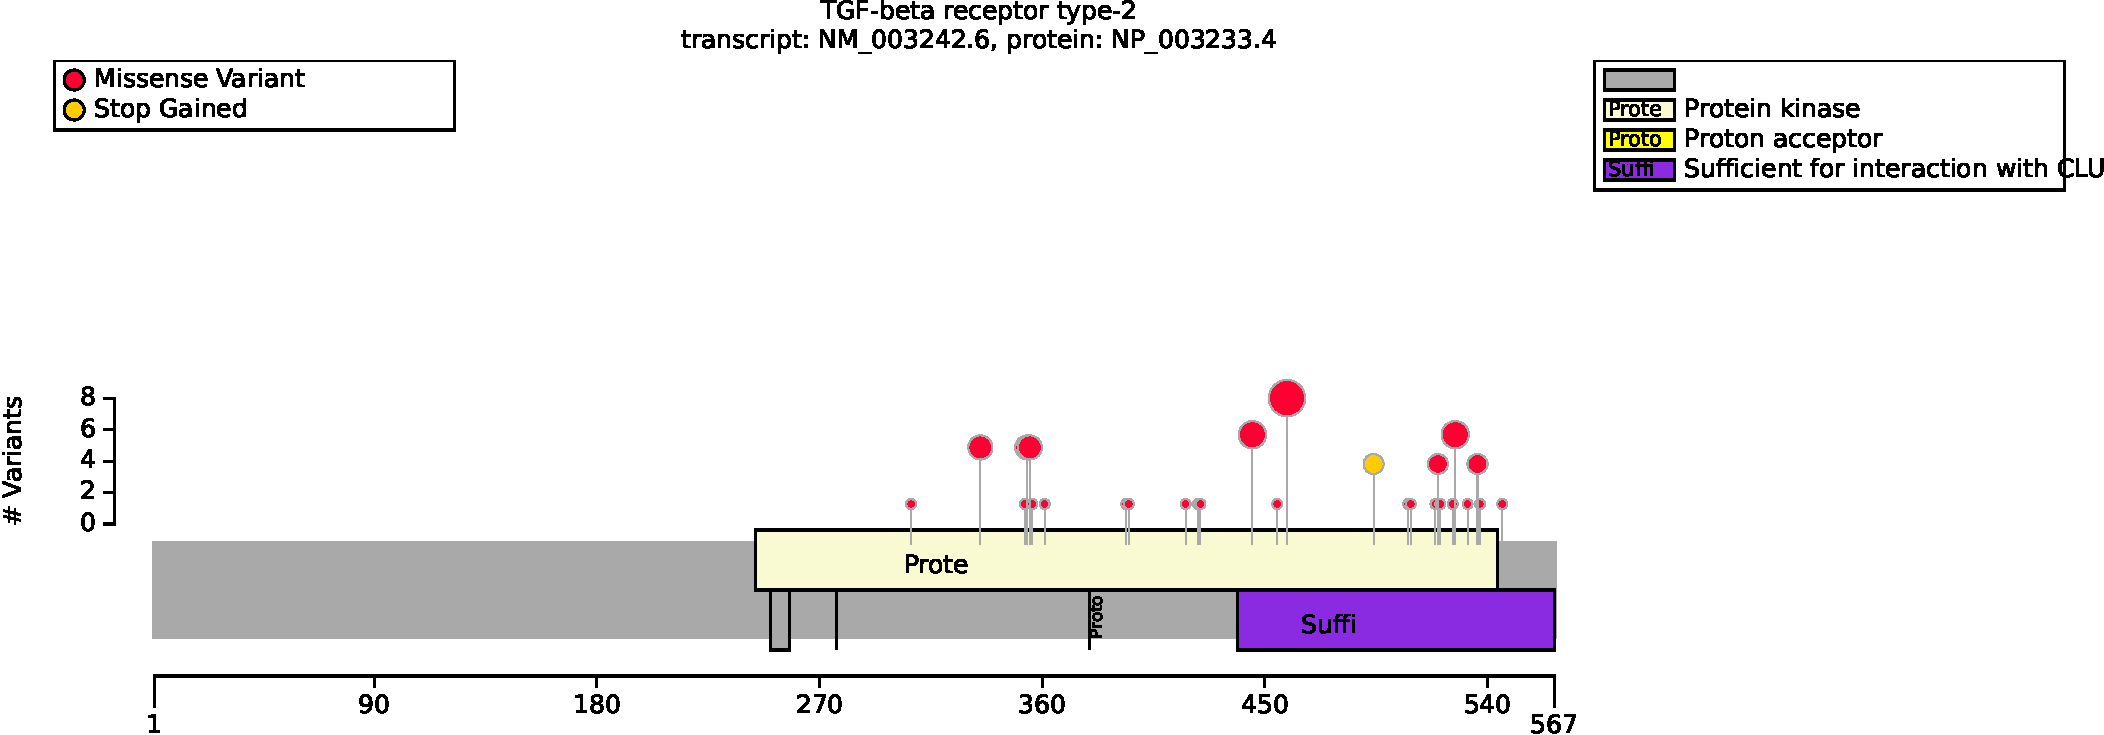
\includegraphics[width=\textwidth]{ img/TGFBR2_protein_diagram.pdf} 
\captionsetup{justification=raggedright,singlelinecheck=false}
\caption{Distribution of variants in TGFBR2}
\end{subfigure}

\vspace{2em}

\begin{subfigure}[b]{0.95\textwidth}
\centering
\resizebox{\textwidth}{!}{
\begin{tabular}{llllrr}
\toprule
Genotype (A) & Genotype (B) & total tests performed & significant results\\
\midrule
CLU interaction region & Other & 37 & 0\\
Missense & Other & 37 & 0\\
FEMALE & MALE & 35 & 0\\
\bottomrule
\end{tabular}
}
\captionsetup{justification=raggedright,singlelinecheck=false}
\caption{Fisher Exact Test performed to compare HPO annotation frequency with respect to genotypes.}
\end{subfigure}

\vspace{2em}

\caption{The cohort comprised 53 individuals (23 females, 30 males). 4 of these individuals were reported to be deceased. A total of 96 HPO terms were used to annotate the cohort. Disease diagnosis: Loeys-Dietz syndrome 2 (OMIM:610168). No statistically significant results identified. A total of 53 unique variant alleles were found in \textit{TGFBR2} (transcript: \texttt{NM\_003242.6}, protein id: \texttt{NP\_003233.4}).}
\end{figure}

\begin{figure}[htbp]
\section*{ TRAF7}
\centering
\begin{subfigure}[b]{0.95\textwidth}
\centering
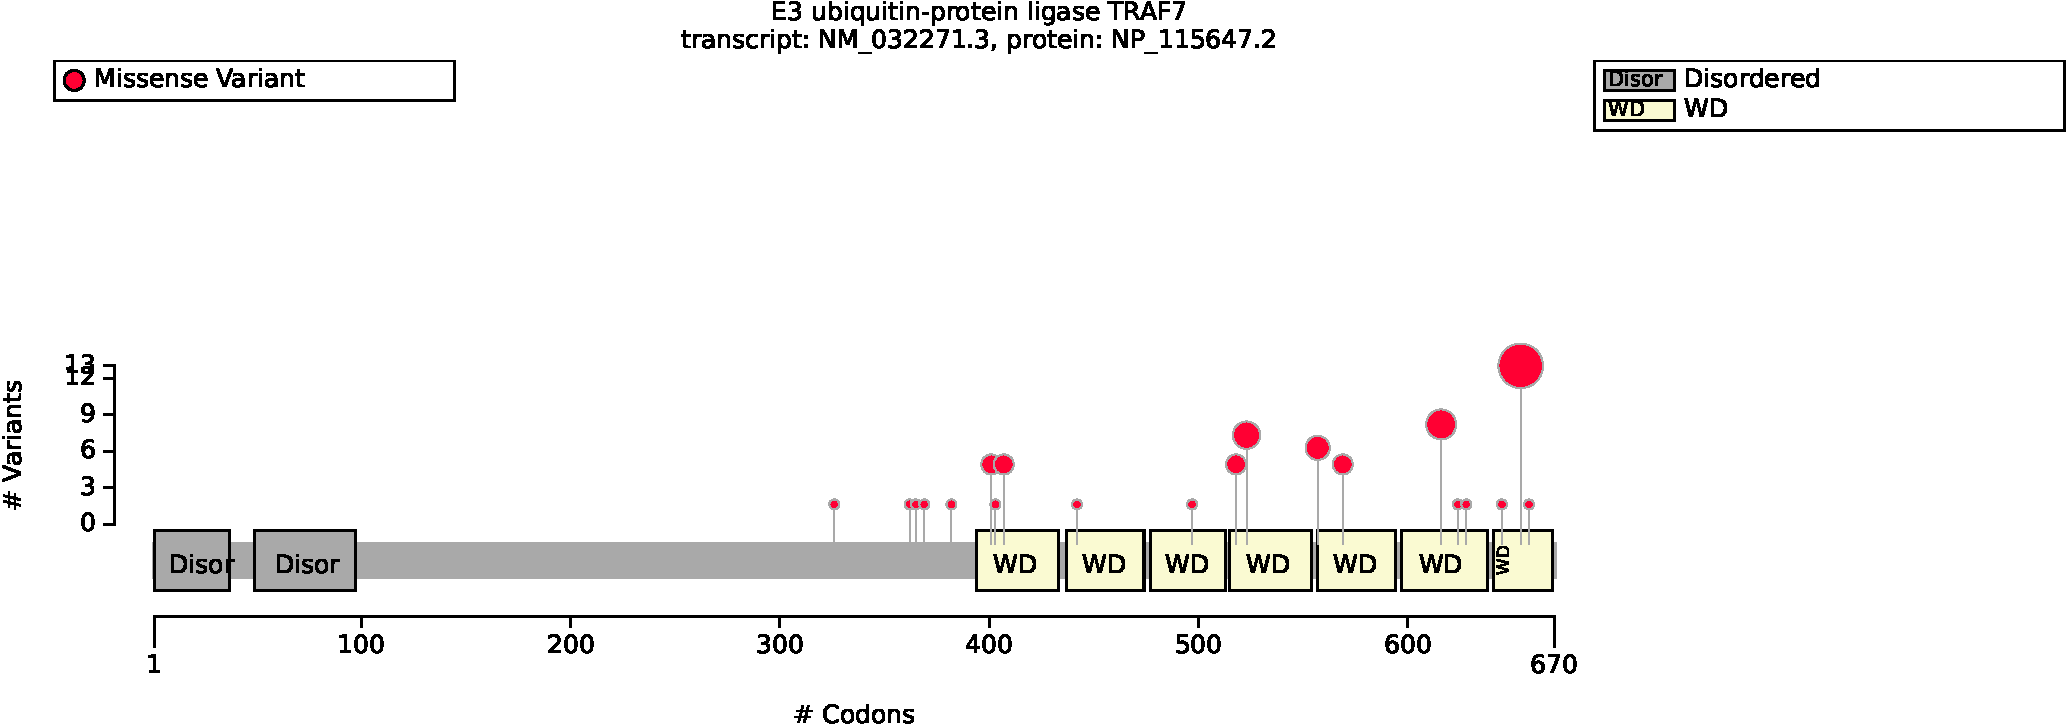
\includegraphics[width=\textwidth]{ img/TRAF7_protein_diagram.pdf} 
\captionsetup{justification=raggedright,singlelinecheck=false}
\caption{Distribution of variants in TRAF7}
\end{subfigure}

\vspace{2em}

\begin{subfigure}[b]{0.95\textwidth}
\centering
\resizebox{\textwidth}{!}{
\begin{tabular}{llllrr}
\toprule
Genotype (A) & Genotype (B) & total tests performed & significant results\\
\midrule
WD7 & other & 35 & 0\\
Arg655Gln & Other variant & 35 & 0\\
FEMALE & MALE & 35 & 0\\
\bottomrule
\end{tabular}
}
\captionsetup{justification=raggedright,singlelinecheck=false}
\caption{Fisher Exact Test performed to compare HPO annotation frequency with respect to genotypes.}
\end{subfigure}

\vspace{2em}

\caption{ The cohort comprised 45 individuals (17 females, 28 males). A total of 360 HPO terms were used to annotate the cohort. Disease diagnosis: Cardiac, facial, and digital anomalies with developmental delay (OMIM:618164). No significant correlations identified. A total of 45 unique variant alleles were found in \textit{TRAF7} (transcript: \texttt{NM\_032271.3}, protein id: \texttt{NP\_115647.2}).}
\end{figure}

\bibliography{references}
\bibliographystyle{unsrt}


\end{document}
